\documentclass[11pt]{article}

\usepackage[preprint]{acl}
\usepackage{times}
\usepackage{latexsym}
\usepackage[T1]{fontenc}
\usepackage[utf8]{inputenc}
\usepackage{microtype}
\usepackage{inconsolata}
\usepackage{graphicx}
\usepackage{booktabs}
\usepackage{amsmath}
\usepackage{amssymb}
\usepackage{xcolor}
\usepackage{enumitem}
\usepackage{placeins}
\renewcommand{\topfraction}{0.9}
\renewcommand{\dbltopfraction}{0.9}
\renewcommand{\textfraction}{0.07}
\renewcommand{\floatpagefraction}{0.75}
\renewcommand{\dblfloatpagefraction}{0.75}
\setcounter{topnumber}{4}
\setcounter{dbltopnumber}{3}
\setcounter{totalnumber}{6}
\setlist{nosep,leftmargin=*}

\newcommand{\sem}{s_{\mathit{sem}}}
\newcommand{\ctx}{s_{\mathit{ctx}}}
\newcommand{\gate}[1]{\textsc{#1}}

\title{Does the Fusion Weight Track Query Complexity?\\
Adaptive Score Fusion of Cross-Encoder and Graph-Contextual Evidence\\ for Single- and Multi-hop Passage Ranking}

\author{Anonymous Authors \\
  \texttt{(author information to be added)}}

\begin{document}
\maketitle

\begin{abstract}
Graph-augmented rerankers such as ReGAT-BERT score a passage with a linear fusion
$\alpha\,\sem + (1-\alpha)\,\ctx$ of a cross-encoder score $\sem$ and a contextual score $\ctx$
produced by a graph attention network (GAT) over the candidate set, with one global $\alpha$.
We test a natural hypothesis: \emph{simple, single-hop queries should rely on the cross-encoder
($\alpha>0.5$), complex multi-hop queries on the contextual score ($\alpha<0.5$), so an $\alpha$ that
depends on the query should beat a fixed one.} We ablate four score normalisers and five ways of
setting $\alpha$ (fixed; a function of the query, of score statistics, or of both; plus explicit
complexity features) on MS MARCO and four multi-hop collections (MuSiQue, HotpotQA, BEIR-HotpotQA,
2WikiMultiHopQA), with every upstream model frozen and all selection on validation data.
The hypothesis holds in a qualified form. The best fixed $\alpha$ is above 0.5 on MS MARCO and
falls below 0.5 on 2WikiMultiHopQA, on MuSiQue's validation split and on its 4-hop test questions;
within MuSiQue the test optimum falls with the hop count (0.80, 0.55, 0.40 for 2, 3, 4 hops), and
within 2WikiMultiHopQA comparison questions favour the cross-encoder while bridge-comparison and
inference questions favour the GAT. Across 17 query buckets, however, the optimum is explained by
the relative strength of the two signals (Spearman $\rho=0.79$ with the CE$-$GAT gap) rather than by
complexity as such: on HotpotQA, bridge questions favour the cross-encoder.
The second half of the hypothesis is not supported by learned gates: although a per-query oracle
$\alpha$ would add 2.3--7.4 nDCG@10 points, the query-dependent gates gain at most 0.04 points over the
fixed weight under the primary normaliser (11 of 76 gate/normaliser/dataset cells significantly
better, 13 worse), mostly because early stopping returns their constant initialisation. A coarse
question-type $\alpha$ chosen on validation data gives small significant gains (up to +0.42).
\end{abstract}

% =====================================================================
\section{Introduction}
\label{sec:intro}

Neural rerankers increasingly combine a pointwise relevance model with evidence drawn from the
other candidates: graph-based score regularisation \citep{diaz2005regularizing,kurland2005pagerank},
corpus-graph reranking \citep{macavaney2022gar}, and graph-attention models over passages and their
links \citep{asai2020learning}. ReGAT-BERT \citep{regatbert} is one such design. A BERT
cross-encoder \citep{nogueira2019passage} gives a semantic score $\sem(q,p)$; a GAT
\citep{velickovic2018gat} refines bi-encoder passage embeddings over a graph of candidates, and
the cosine with the query gives a contextual score $\ctx(q,p)$. The final score is
\begin{equation}
  \label{eq:fusion}
  s(q,p) = \alpha\, \sem(q,p) + (1-\alpha)\, \ctx(q,p),
\end{equation}
with a single $\alpha$ for all queries.

A single weight is a strong assumption. A single-hop query (``\emph{what is the capital of
Peru}'') can be answered by a passage judged in isolation, so the cross-encoder should dominate.
A multi-hop question (``\emph{who directed the film whose lead actress was born in Lima}'') needs
passages that are only relevant through their relation to other passages, which is exactly what
a graph over the candidate set can encode. This suggests the hypothesis we test:

\begin{quote}
\textbf{Hypothesis.} For simple single-hop queries $\alpha>0.5$ (the semantic score matters more);
for complex multi-hop queries $\alpha<0.5$ (the contextual score matters more). Hence $\alpha$
should depend on the query, and an $\alpha$ conditioned on the query (\gate{Q}), on the query and
the score distributions (\gate{QS}) or on the score distributions alone (\gate{S}) should beat a
fixed $\alpha$.
\end{quote}

We split the hypothesis into falsifiable claims and test them in a controlled ablation in which
only the fusion step changes (\S\ref{sec:setup}). The BM25 candidates, the cross-encoder, the
bi-encoder and the GAT are trained or loaded once, frozen and cached, so every fusion variant sees
identical inputs. Our contributions are:
\begin{itemize}
\item A $4\times5$ ablation of fusion (normaliser $\times$ what $\alpha$ depends on) on MS MARCO
  and four multi-hop collections, with oracle upper bounds, graph controls, transfer experiments
  and pre-registered hypothesis tests (written down before any multi-hop run).
\item Evidence that the \emph{optimal} fusion weight does vary with query complexity in the predicted
  direction on the hardest multi-hop data (MuSiQue, 2WikiMultiHopQA), but that it is governed by the
  relative reliability of the two signals ($\rho=0.79$ across buckets), which complexity
  only partly determines (\S\ref{sec:dataset}, \S\ref{sec:query}).
\item Evidence that learned query-dependent gates do not realise this variation: they collapse to
  the fixed weight, and the few significant gains are either tiny or repair a weak normaliser
  (\S\ref{sec:gates}). We trace this to early stopping, weak per-query signal and a train/val shift.
\end{itemize}

% =====================================================================
\section{Related Work}
\label{sec:related}

\paragraph{Score fusion and normalisation.}
Linear combination of retrieval scores goes back to CombSUM and its variants
\citep{fox1994combination}; because scores live on different scales, per-query normalisation
(min--max, z-score) is standard \citep{montague2001normalization}, and rank-based fusion such as
RRF \citep{cormack2009rrf} avoids scores altogether. We compare four normalisers because the
numerical value of $\alpha$ is only meaningful relative to the scales of $\sem$ and $\ctx$.

\paragraph{Graph-based and contextual reranking.}
Score regularisation smooths scores over a document-similarity graph \citep{diaz2005regularizing};
structural reranking uses graphs induced by language models \citep{kurland2005pagerank}; adaptive
reranking expands the candidate pool through a corpus graph \citep{macavaney2022gar}. ReGAT-BERT
\citep{regatbert} learns the propagation with a GAT and fuses it with a cross-encoder through a fixed
weight, the component we study. We use GATv2 layers \citep{brody2022gatv2} implemented in PyTorch
Geometric \citep{fey2019pyg}.

\paragraph{Multi-hop retrieval.}
Multi-hop QA datasets \citep{yang2018hotpotqa,ho2020constructing,trivedi2022musique} require
combining several supporting paragraphs; retrievers for them follow hyperlinks or retrieve
iteratively \citep{asai2020learning,xiong2021mdr}. Many HotpotQA questions can be answered with
single-hop shortcuts \citep{min2019compositional}, which motivated MuSiQue's construction
\citep{trivedi2022musique}; this matters for our results on HotpotQA (\S\ref{sec:query}).

% =====================================================================
\section{Hypotheses and Tests}
\label{sec:hyp}

The hypothesis in \S\ref{sec:intro} makes three claims, which we test separately.
\begin{description}
\item[C1 (dataset level).] On single-hop data the best fixed $\alpha$ exceeds 0.5; on multi-hop data
  it is below 0.5.
\item[C2 (query level).] Within a dataset, the best $\alpha$ falls as complexity rises (more hops;
  bridge or inference rather than comparison questions).
\item[C3 (method).] A query-dependent gate (\gate{Q}, \gate{QS}, \gate{S}) beats the best fixed
  $\alpha$, and gains more on multi-hop than on single-hop data.
\end{description}
Before running any multi-hop experiment we also fixed four formal hypotheses and their statistics
(Table~\ref{tab:hyp}): \textbf{H1}, the gate's learned $\alpha$ decreases with complexity (Spearman
with hop count on MuSiQue; bridge minus comparison on HotpotQA and BEIR-HotpotQA);
\textbf{H2}, the adaptive gain is larger than on MS MARCO; \textbf{H3}, the oracle headroom is larger
than on MS MARCO; \textbf{H4}, effects that come from the graph should vanish with a random or empty
graph. H1--H3 on the three primary multi-hop datasets form one Holm family \citep{holm1979simple};
everything else is labelled exploratory.

\paragraph{Interpretation rule.} $\alpha$ measures the \emph{relative reliability} of the two
normalised signals, not ``how much context a query needs''. We therefore never read raw $\alpha$ without
the CE-only and GAT-only effectiveness of the same queries and the normaliser it was obtained with.

% =====================================================================
\section{Experimental Setup}
\label{sec:setup}

\subsection{Frozen pipeline}
\textbf{Candidates.} MS MARCO and BEIR-HotpotQA use BM25 (Pyserini, $k_1{=}0.9$, $b{=}0.4$;
\citealp{robertson2009bm25,lin2021pyserini}) top-100. MuSiQue, HotpotQA (distractor) and 2Wiki are
closed pools of 20 or 10 paragraphs that always contain the gold paragraphs; we order each pool by
in-pool BM25, which is also the tie-breaker everywhere.
\textbf{Semantic score.} $\sem$ is the raw logit of \texttt{cross-encoder/ms-marco-MiniLM-L-6-v2}
\citep{wang2020minilm}, never fine-tuned; on multi-hop data the passage is ``\emph{title}. \emph{text}''.
\textbf{Contextual score.} Node features are frozen \texttt{msmarco-MiniLM-L6-cos-v5} embeddings
\citep{reimers2019sbert}. For each query we build a graph over its candidates only (the query is not
a node): a symmetrised $k$-NN graph on cosine similarity ($k{=}8$ for $K{=}100$, $k{=}3$ for closed
pools, minimum cosine 0.3) with self-loops. Two GATv2 layers (4$\times$128 heads, then 384) with a
residual connection and LayerNorm refine the embeddings, and $\ctx$ is the cosine between the query
embedding and the refined passage embedding. One GAT per dataset is trained once on a disjoint
\emph{GAT-train} split with a multi-positive listwise InfoNCE loss ($\tau{=}0.05$;
\citealp{oord2018cpc}), early-stopped on validation, and frozen. A gate checks that GAT-only is not
worse than the raw bi-encoder on validation; it passes on every dataset.

\subsection{Fusion variants}
\textbf{Normalisers} (per query over its candidates): \emph{none}, \emph{min--max}, \emph{z-score},
\emph{rank}. The primary normaliser, fixed on MS MARCO validation before any multi-hop run, is
min--max.
\textbf{What $\alpha$ depends on.}
\gate{Fixed}: a grid search $\alpha\in\{0,0.05,\dots,1\}$ on validation (main baseline, $\alpha_0$)
and a learned scalar.
\gate{Q}: $\alpha=\sigma(\mathrm{MLP}(\mathbf{q}))$ on the query embedding.
\gate{S}: $\alpha=\sigma(\mathrm{MLP}(\mathbf{f}))$ on 12 statistics of the raw score lists (mean, std,
max, top-1/top-2 gap and softmax entropy of each score; Spearman correlation and top-$m$ overlap
between them).
\gate{QS}: both inputs. \gate{QS+C}: \gate{QS} plus query length and spaCy entity count.
Each MLP has one hidden layer of 64 units, its output bias is initialised to $\mathrm{logit}(\alpha_0)$
and its last-layer weights near zero, so every gate starts as the fixed baseline.
\textbf{Training.} Gates are trained on a disjoint \emph{fusion-train} split with a multi-positive
listwise softmax loss \citep{cao2007listnet} on $s/T$ (learned temperature), plus
$\lambda(\alpha-\alpha_0)^2$ with $\lambda{=}0.01$ (and $\lambda{=}0$ as an ablation), AdamW
\citep{loshchilov2019adamw}, early stopping on validation nDCG@10 with the best epoch restored
(epoch 0 = the initialisation), 5 seeds.
\textbf{ReGAT-BERT-style row}: $a\,\sem + b\,\ctx$ with free $a,b$ trained with pointwise BCE, our
reproduction of the original training objective.
\textbf{Oracle}: the per-query $\alpha$ on the grid that maximises that query's test nDCG@10; an upper
bound, not a method.

\subsection{Data}
Table~\ref{tab:data} lists the collections. MS MARCO is used under two protocols: \textbf{A} trains on
MS MARCO train and tests on dev/small; \textbf{B} splits dev/small itself, so neither the GAT nor the
gate's validation data shares a distribution with the cross-encoder's training data. Complexity
labels: MuSiQue hop count (2--4), HotpotQA and BEIR-HotpotQA question type (bridge vs.\ comparison;
BEIR queries joined to HotpotQA by id), 2Wiki question type (comparison, compositional, inference,
bridge-comparison), and for MS MARCO only rule-based proxies (length, wh-word, entities).
Labels never enter a gate.

\begin{table*}[t]
\centering\small
\resizebox{\textwidth}{!}{%
\begin{tabular}{llrrrrrrl}
\toprule
Dataset & Setting & $K$ & GAT train & Fusion train & Val & Test & Gold/pool & Complexity labels \\
\midrule
MS MARCO (A) & open (BM25) & 100 & 30,000 & 10,000 & 2,000 & 6,980 & -- & proxies only \\
MS MARCO (B) & open (BM25) & 100 & 1,870 & 1,150 & 698 & 1,745 & -- & proxies only \\
MuSiQue & closed pool & 20 & 10,000 & 7,000 & 2,938 & 2,417 & 2.65 & hops 2/3/4 \\
HotpotQA & closed pool & 10 & 20,000 & 10,000 & 2,000 & 7,405 & 2.00 & bridge/comparison \\
BEIR-HotpotQA & open (BM25) & 100 & 20,000 & 10,000 & 2,000 & 7,405 & 1.59 & bridge/comparison \\
2Wiki & closed pool & 10 & 20,000 & 10,000 & 2,000 & 12,576 & 2.44 & 4 types \\
\bottomrule
\end{tabular}}
\caption{Datasets and splits (queries). Val is always carved from the training data; test is the official dev set (MS MARCO A: dev/small; MuSiQue, HotpotQA, 2Wiki: dev; BEIR: test). MS MARCO B splits dev/small itself, so the cross-encoder never saw any of its queries. Gold/pool = mean number of relevant passages among the $K$ test candidates.}
\label{tab:data}
\end{table*}


\subsection{Evaluation}
We report nDCG, MRR, Precision and Recall at $k\in\{1,3,5,10,50\}$, MAP, and AllRecall@$k$ (all
gold paragraphs in the top $k$), computed with ir\_measures \citep{macavaney2022irmeasures}; nDCG@10 is
the primary metric (full tables in Appendix~\ref{app:full}). Every choice ($\alpha_0$, early stopping,
the primary normaliser) is made on validation data; test sets are used once. Differences are tested with
a paired bootstrap over queries (10{,}000 resamples; \citealp{efron1993bootstrap}) on seed-averaged
per-query scores.

% =====================================================================
\section{Results}
\label{sec:results}

\begin{table*}[t]
\centering\small\setlength{\tabcolsep}{3.2pt}
\resizebox{\textwidth}{!}{%
\begin{tabular}{lrrrrrrrrrrrr}
\toprule
 & \multicolumn{2}{c}{MSM-A} & \multicolumn{2}{c}{MSM-B} & \multicolumn{2}{c}{MuSiQue} & \multicolumn{2}{c}{HotpotQA} & \multicolumn{2}{c}{BEIR-HQA} & \multicolumn{2}{c}{2Wiki} \\
\cmidrule(lr){2-3} \cmidrule(lr){4-5} \cmidrule(lr){6-7} \cmidrule(lr){8-9} \cmidrule(lr){10-11} \cmidrule(lr){12-13}
 & nDCG & MRR & nDCG & MRR & nDCG & MRR & nDCG & MRR & nDCG & MRR & nDCG & MRR \\
\midrule
BM25 (first stage / in-pool) & 22.84 & 18.40 & 22.96 & 18.51 & 55.11 & 75.70 & 81.74 & 87.87 & 63.29 & 80.32 & 87.77 & 96.51 \\
SBERT ($s_{bi}$) & 35.30 & 30.38 & 35.74 & 30.86 & 67.08 & 81.83 & 82.94 & 87.19 & 53.67 & 70.29 & 89.19 & 96.89 \\
CE only ($\alpha{=}1$) & 41.34 & 36.39 & 41.54 & 36.58 & 71.09 & 87.32 & 89.84 & 95.42 & 72.61 & 89.02 & 90.77 & 98.16 \\
GAT only ($\alpha{=}0$) & 35.42 & 30.43 & 35.70 & 30.58 & 66.81 & 81.48 & 84.14 & 88.39 & 55.47 & 72.63 & 91.00 & 97.54 \\
\midrule
ReGAT-BERT-style ($a,b$; BCE) & 39.83$^{\triangledown}$ & 34.72$^{\triangledown}$ & 40.25$^{\triangledown}$ & 35.22$^{\triangledown}$ & 71.74$^{\blacktriangle}$ & 87.29$^{\blacktriangle}$ & 89.89 & 95.35 & 68.81$^{\triangledown}$ & 85.35$^{\triangledown}$ & 91.73 & 98.56 \\
Fixed $\alpha$ (grid on val) & 40.89 & 35.86 & 41.69 & 36.84 & 71.28 & 86.28 & 89.87 & 95.28 & 72.63 & 89.03 & 91.75 & 98.54 \\
Fixed $\alpha$ (learned) & 40.89 & 35.86 & 41.69 & 36.84 & 71.28 & 86.28 & 89.89 & 95.32 & 72.63 & 89.03 & 91.75 & 98.54 \\
\midrule
Adaptive $\alpha(q)$ \textsc{Q} & 40.89$^{\blacktriangle}$ & 35.87 & 41.70 & 36.83 & 71.28 & 86.28 & 89.87 & 95.28 & 72.63 & 89.03 & 91.77 & 98.37$^{\triangledown}$ \\
Adaptive $\alpha(q,s)$ \textsc{QS} & 40.89 & 35.86 & 41.70 & 36.84 & 71.27 & 86.28 & 89.91 & 95.49 & 72.63 & 89.03 & 91.63$^{\triangledown}$ & 98.40$^{\triangledown}$ \\
Adaptive $\alpha(s)$ \textsc{S} & 40.90 & 35.87 & 41.71$^{\blacktriangle}$ & 36.86 & 71.27 & 86.31 & 89.93 & 95.49$^{\blacktriangle}$ & 72.64 & 89.03 & 91.75 & 98.53 \\
Adaptive \textsc{QS+C} & -- & -- & -- & -- & 71.28 & 86.28 & 89.92 & 95.52$^{\blacktriangle}$ & 72.63 & 89.03 & 91.63$^{\triangledown}$ & 98.35$^{\triangledown}$ \\
\midrule
\textit{Oracle per-query $\alpha$ (bound)} & 45.90 & 41.81 & 46.01 & 41.95 & 78.72 & 92.50 & 92.86 & 97.69 & 75.56 & 92.04 & 94.00 & 99.49 \\
\bottomrule
\end{tabular}}
\caption{Main results on the test sets (nDCG@10 and MRR@10, $\times 100$, mean over 5 seeds) under the primary normaliser (min--max, fixed on MS MARCO val). $^{\blacktriangle}$/$^{\triangledown}$: significantly better/worse than the best fixed $\alpha$ (paired bootstrap over queries, 10k resamples, $p<0.05$, uncorrected). The oracle row picks $\alpha$ per query on the test labels and is an upper bound, not a method. \gate{QS+C} was added with the multi-hop extension and not run on MS MARCO (--). Full metrics at $k\in\{1,3,5,10,50\}$ are in Appendix~\ref{app:full}.}
\label{tab:main}
\end{table*}


\subsection{Overall effectiveness}
Table~\ref{tab:main} shows the headline numbers. Fusion helps little over the cross-encoder alone:
the best fixed $\alpha$ adds +0.98 nDCG@10 on 2Wiki, where the GAT is as strong as the cross-encoder,
+0.19 on MuSiQue and +0.15 on MS MARCO B, and is \emph{below} CE-only on MS MARCO A (40.89 vs.\ 41.34)
because the $\alpha_0$ chosen on validation (0.70) is far from the test optimum (0.95;
\S\ref{sec:dataset}). The ReGAT-BERT-style free-weight BCE row is significantly worse than the fixed
$\alpha$ on MS MARCO and BEIR-HotpotQA ($-1.1$ and $-3.8$) and significantly better on MuSiQue
(+0.46). The adaptive gates gain at most 0.04 points over the fixed $\alpha$ on any dataset, and \gate{QS} loses
0.12 on 2Wiki.
The oracle rows show what a perfect per-query weight could achieve: +2.3 (2Wiki) to +7.4 (MuSiQue)
nDCG@10 points, so the lack of gains is not due to a lack of headroom.

% ---------------------------------------------------------------------
\subsection{C1: Is $\alpha$ below 0.5 on multi-hop data?}
\label{sec:dataset}

\begin{figure*}[t]
  \centering
  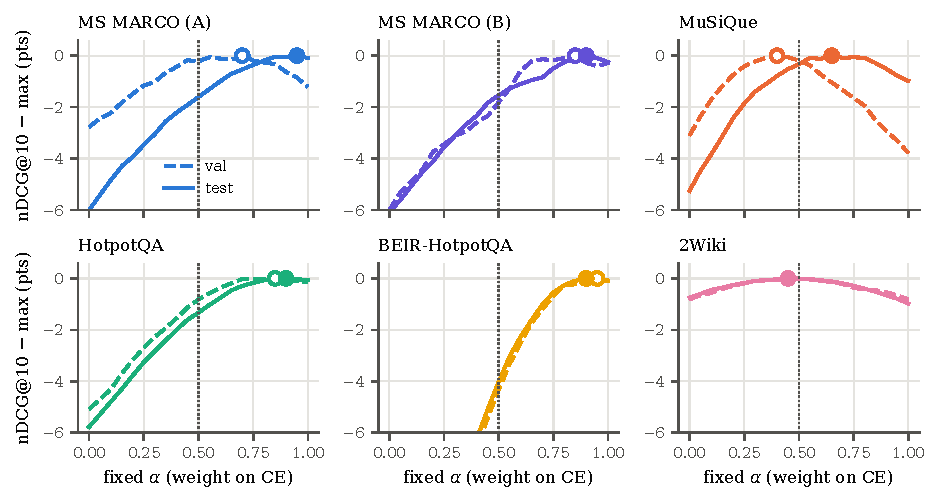
\includegraphics[width=\textwidth]{figures/alpha_curves.pdf}
  \caption{nDCG@10 as a function of the fixed fusion weight $\alpha$ (min--max), relative to each
  curve's maximum; dashed = validation, solid = test, circles = arg-max. Left of the dotted line the
  GAT score has more weight. The y-axis is clipped at $-6$ points.}
  \label{fig:curves}
\end{figure*}

\begin{table*}[t]
\centering\small\setlength{\tabcolsep}{4pt}
\begin{tabular}{lrrrrrrrrrc}
\toprule
 & \multicolumn{3}{c}{Test nDCG@10 ($\times$100)} & \multicolumn{4}{c}{Best fixed $\alpha$ on val, by normaliser} & \multicolumn{2}{c}{min--max $\alpha^*$} & \\
\cmidrule(lr){2-4}\cmidrule(lr){5-8}\cmidrule(lr){9-10}
Dataset & CE & GAT & CE$-$GAT & none & min--max & z-score & rank & val & test & favours \\
\midrule
MS MARCO (A) & 41.3 & 35.4 & +5.9 & 0.05 & 0.70 & 0.70 & 0.55 & \textbf{0.70} & 0.95 & sem/sem \\
MS MARCO (B) & 41.5 & 35.7 & +5.8 & 0.15 & 0.85 & 0.85 & 1.00 & \textbf{0.85} & 0.90 & sem/sem \\
MuSiQue & 71.1 & 66.8 & +4.3 & 0.05 & 0.40 & 0.45 & 0.45 & \textbf{0.40} & 0.65 & ctx/sem \\
HotpotQA & 89.8 & 84.1 & +5.7 & 0.10 & 0.85 & 0.85 & 0.90 & \textbf{0.85} & 0.90 & sem/sem \\
BEIR-HotpotQA & 72.6 & 55.5 & +17.1 & 0.35 & 0.95 & 0.95 & 1.00 & \textbf{0.95} & 0.90 & sem/sem \\
2Wiki & 90.8 & 91.0 & -0.2 & 0.05 & 0.45 & 0.50 & 0.55 & \textbf{0.45} & 0.45 & ctx/ctx \\
\bottomrule
\end{tabular}
\caption{Dataset-level test of the hypothesis. $\alpha$ weights the cross-encoder: fused $=\alpha\, s_{sem} + (1-\alpha)\, s_{ctx}$. $\alpha^*$ is the arg-max of mean nDCG@10 over the grid $\{0,0.05,\dots,1\}$; the val value (bold) is the one used by the fixed baseline, the test value is for analysis only. ``favours'': ctx if $\alpha^*<0.5$, sem if $\alpha^*>0.5$ (val/test). With raw scores (none) $\alpha$ mostly reflects the scale ratio of the two scores and is not interpretable.}
\label{tab:dsalpha}
\end{table*}


Table~\ref{tab:dsalpha} and Figure~\ref{fig:curves} give the best fixed $\alpha$ per dataset.
With raw scores (``none'') $\alpha$ only reflects the ratio of score scales (within a query, cross-encoder logits span
about 12 units on average, GAT cosines about 0.5) and is near 0 everywhere, so the claim can only be read under a
scale-free normaliser. Under min--max and z-score:
\begin{itemize}
\item \textbf{MS MARCO} favours the cross-encoder: $\alpha^*=0.70$ (A) and 0.85 (B) on validation, 0.95
  and 0.90 on test. This agrees with C1.
\item \textbf{2Wiki} favours the GAT: $\alpha^*=0.45$ on validation and test (0.50 under z-score), the only
  dataset where GAT-only matches CE-only (91.0 vs.\ 90.8).
\item \textbf{MuSiQue} favours the GAT on validation ($\alpha^*=0.40$) but the cross-encoder on test (0.65).
\item \textbf{HotpotQA} and \textbf{BEIR-HotpotQA} favour the cross-encoder strongly (0.85--0.95),
  contrary to C1.
\end{itemize}
The MuSiQue and MS MARCO-A shifts between validation and test have the same cause. Both validation sets
are carved from the training questions, i.e.\ from the same distribution as the GAT's training data,
whereas the test sets are the official dev sets. The GAT is relatively stronger on validation
(MuSiQue: CE$-$GAT $=-0.7$ points on val vs.\ $+4.3$ on test; MS MARCO A: $+1.6$ vs.\ $+5.9$), so
validation asks for more GAT weight. Protocol B, whose validation and test both come from dev/small,
has no such shift (gap $+5.7$ vs.\ $+5.8$; $\alpha^*$ 0.85 vs.\ 0.90). \textbf{C1 therefore holds for
the two hardest multi-hop collections (2Wiki; MuSiQue in-distribution) and fails for HotpotQA.}

% ---------------------------------------------------------------------
\subsection{C2: Does the best $\alpha$ fall with complexity?}
\label{sec:query}

\begin{figure}[t]
  \centering
  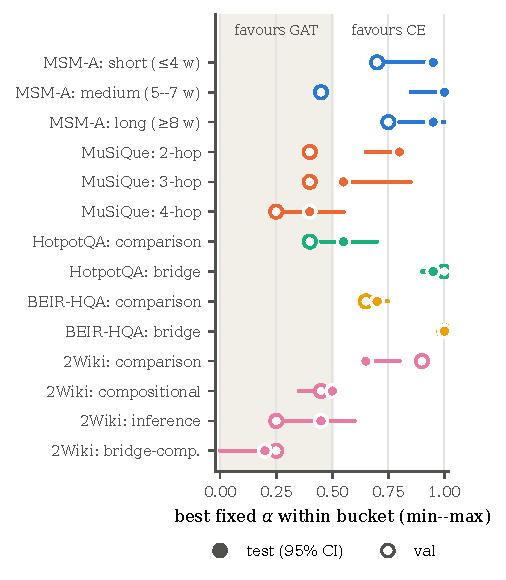
\includegraphics[width=\columnwidth]{figures/bucket_alpha.pdf}
  \caption{Best fixed $\alpha$ within each complexity bucket (min--max). Filled: test with 95\%
  bootstrap CI; open: validation. Shaded: the GAT score has more weight.}
  \label{fig:buckets}
\end{figure}

\begin{table*}[t]
\centering\small\setlength{\tabcolsep}{4pt}
\begin{tabular}{llrrrrlrr}
\toprule
 & & & \multicolumn{2}{c}{Test nDCG@10} & \multicolumn{2}{c}{Best fixed $\alpha$ in bucket} & \% queries & Learned \\
\cmidrule(lr){4-5}\cmidrule(lr){6-7}
Dataset & Bucket & $n$ (test) & CE & GAT & val & test [95\% CI] & prefer ctx & $\bar\alpha$ (gate) \\
\midrule
MS MARCO (A) & short ($\le$4 w) & 2,149 & 45.0 & 40.3 & 0.70 & 0.95 [0.70, 0.95] & 35 & -- \\
 & medium (5--7 w) & 3,291 & 41.6 & 35.3 & 0.45 & 1.00 [0.85, 1.00] & 33 & -- \\
 & long ($\ge$8 w) & 1,540 & 35.8 & 28.8 & 0.75 & 0.95 [0.80, 1.00] & 31 & -- \\
\midrule
MuSiQue & 2-hop & 1,252 & 73.8 & 68.0 & 0.40 & 0.80 [0.65, 0.80] & 40 & 0.40 \\
 & 3-hop & 760 & 71.8 & 66.7 & 0.40 & 0.55 [0.55, 0.85] & 39 & 0.40 \\
 & 4-hop & 405 & 61.3 & 63.3 & 0.25 & 0.40 [0.25, 0.55] & 52 & 0.40 \\
\midrule
HotpotQA & comparison & 1,487 & 95.6 & 94.4 & 0.40 & 0.55 [0.45, 0.70] & 40 & 0.90 \\
 & bridge & 5,918 & 88.4 & 81.6 & 1.00 & 0.95 [0.90, 1.00] & 33 & 0.88 \\
\midrule
BEIR-HotpotQA & comparison & 1,487 & 85.7 & 77.2 & 0.65 & 0.70 [0.65, 0.75] & 27 & 0.95 \\
 & bridge & 5,918 & 69.3 & 50.0 & 1.00 & 1.00 [1.00, 1.00] & 12 & 0.95 \\
\midrule
2Wiki & comparison & 3,040 & 97.3 & 95.5 & 0.90 & 0.65 [0.65, 0.80] & 30 & 0.72 \\
 & bridge-comp. & 2,751 & 90.1 & 92.0 & 0.25 & 0.20 [0.00, 0.20] & 67 & 0.35 \\
 & compositional & 5,236 & 88.5 & 88.9 & 0.45 & 0.50 [0.35, 0.50] & 53 & 0.45 \\
 & inference & 1,549 & 86.7 & 87.6 & 0.25 & 0.45 [0.25, 0.60] & 59 & 0.30 \\
\bottomrule
\end{tabular}
\caption{Query-level test of the hypothesis (min--max). Best fixed $\alpha$ = arg-max of the bucket's mean nDCG@10 curve; CI from 2{,}000 bootstrap resamples of the bucket's queries. ``\% prefer ctx'': among queries whose nDCG@10 changes with $\alpha$, the share whose optimal $\alpha$-interval is centred below 0.5 (tie-robust; the remaining queries are indifferent). Learned $\bar\alpha$: mean $\alpha$ of the best (on val) in-domain gate in the bucket. Analysis only: no label enters any gate.}
\label{tab:bucket}
\end{table*}


Because a learned gate may fail to find structure that exists, we test C2 directly on the data: for
every bucket we take the $\alpha$ that maximises the bucket's mean nDCG@10, with a bootstrap CI
(Table~\ref{tab:bucket}, Figure~\ref{fig:buckets}).

\textbf{MuSiQue supports C2.} On test the optimum falls monotonically with the hop count:
0.80 [0.65, 0.80] for 2 hops, 0.55 [0.55, 0.85] for 3 hops and 0.40 [0.25, 0.55] for 4 hops (validation:
0.40, 0.40, 0.25). For 4-hop questions the GAT alone beats the cross-encoder (63.3 vs.\ 61.3 nDCG@10),
and 52\% of the 4-hop questions whose ranking depends on $\alpha$ prefer the GAT side, against 40\% of
2-hop questions.

\textbf{2Wiki supports C2.} Comparison questions, whose two gold paragraphs are each named in the
question, have their optimum at 0.65 (val 0.90); compositional questions at 0.50 (0.45); inference at
0.45 (0.25); bridge-comparison questions, which combine a bridge step with a comparison, at 0.20 [0.00,
0.20] (val 0.25), with 67\% of $\alpha$-sensitive queries preferring the GAT side. The GAT beats the
cross-encoder on exactly the three non-comparison types.

\textbf{HotpotQA and BEIR-HotpotQA contradict C2.} Bridge questions, the nominally harder type, have
the higher optimum (0.95--1.00), and comparison questions the lower one (0.55 and 0.70).
Bridge questions are where the cross-encoder's lead over the GAT is largest (6.8 and 19.3 points);
many of them can be solved by matching the question against a single paragraph
\citep{min2019compositional}, while for comparison questions the two gold paragraphs are similar to
each other and therefore close in the $k$-NN graph.

\textbf{MS MARCO} shows no complexity effect: every length bucket has its test optimum at 0.95--1.00,
in line with the Step~0 diagnosis (Appendix~\ref{app:diag}), where learned and oracle $\alpha$ did not
vary with query length, wh-word or entity count.

\begin{figure}[t]
  \centering
  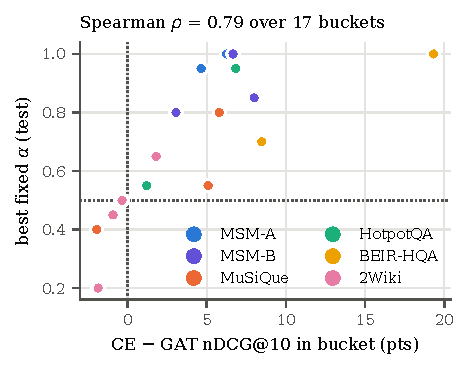
\includegraphics[width=\columnwidth]{figures/gap_vs_alpha.pdf}
  \caption{Each point is one complexity bucket (test): the CE$-$GAT nDCG@10 gap of its queries vs.\ its
  best fixed $\alpha$ (min--max).}
  \label{fig:gap}
\end{figure}

\paragraph{One variable explains the optima.}
Figure~\ref{fig:gap} plots each bucket's optimum against the effectiveness gap between the two
signals on the same queries. The rank correlation is $\rho=0.79$ over 17 buckets from all six test sets:
wherever the GAT is at least as good as the cross-encoder (MuSiQue 4-hop, the three non-comparison 2Wiki
types), the optimum is below 0.5, and it rises towards 1 as the cross-encoder pulls ahead. The same
holds across graphs (Table~\ref{tab:graph}): on HotpotQA, title-link edges raise GAT-only nDCG@10 from
84.1 to 87.4 and move the fixed optimum from 0.85 to 0.65. Query complexity thus matters for $\alpha$
\emph{through} the relative reliability of the two signals: multi-hop questions favour the contextual
score when, and only when, the graph-refined score actually ranks their passages better.

% ---------------------------------------------------------------------
\subsection{C3: Do query-dependent gates beat a fixed $\alpha$?}
\label{sec:gates}

\begin{table*}[t]
\centering\small\setlength{\tabcolsep}{6pt}
\begin{tabular}{llrrrrrr}
\toprule
Norm. & Gate & MSM-A & MSM-B & MuSiQue & HotpotQA & BEIR-HQA & 2Wiki \\
\midrule
none & \textsc{Q} & -0.48$^{\triangledown}$ & +0.01 & +0.00 & -0.00 & -0.00 & +0.00 \\
 & \textsc{QS} & -0.48$^{\triangledown}$ & +0.00 & +0.00 & +0.01 & -0.00$^{\triangledown}$ & +0.00 \\
 & \textsc{S} & -0.49$^{\triangledown}$ & +0.00 & +0.02 & +0.01 & -0.00 & -0.00 \\
\midrule
minmax & \textsc{Q} & \textbf{+0.00$^{\blacktriangle}$} & +0.00 & +0.00 & -0.02 & -0.00 & +0.03 \\
 & \textsc{QS} & +0.00 & +0.01 & -0.01 & +0.02 & +0.00 & -0.12$^{\triangledown}$ \\
 & \textsc{S} & +0.00 & \textbf{+0.02$^{\blacktriangle}$} & -0.00 & +0.04 & +0.01 & +0.00 \\
 & \textsc{QS+C} & -- & -- & +0.00 & +0.03 & -0.00 & -0.11$^{\triangledown}$ \\
\midrule
zscore & \textsc{Q} & +0.01 & \textbf{+0.05$^{\blacktriangle}$} & -0.15$^{\triangledown}$ & +0.06 & \textbf{+0.18$^{\blacktriangle}$} & +0.00 \\
 & \textsc{QS} & \textbf{+0.02$^{\blacktriangle}$} & -0.01 & -0.14$^{\triangledown}$ & +0.00 & -0.01$^{\triangledown}$ & -0.00 \\
 & \textsc{S} & +0.01 & +0.01 & -0.12$^{\triangledown}$ & +0.01 & -0.01 & -0.01$^{\triangledown}$ \\
\midrule
rank & \textsc{Q} & +0.01 & +0.02 & \textbf{+0.43$^{\blacktriangle}$} & -0.01 & -0.01 & \textbf{+0.30$^{\blacktriangle}$} \\
 & \textsc{QS} & -0.12 & -0.04 & \textbf{+1.22$^{\blacktriangle}$} & -0.04 & -0.04$^{\triangledown}$ & \textbf{+0.41$^{\blacktriangle}$} \\
 & \textsc{S} & -0.10 & -0.02 & \textbf{+1.37$^{\blacktriangle}$} & -0.00 & -0.02$^{\triangledown}$ & \textbf{+0.19$^{\blacktriangle}$} \\
\bottomrule
\end{tabular}
\caption{Every adaptive gate against the best fixed $\alpha$ under the same normaliser: test $\Delta$nDCG@10 $\times$100 (paired bootstrap; $^{\blacktriangle}$ significantly better, $^{\triangledown}$ worse, $p<0.05$ uncorrected).}
\label{tab:grid}
\end{table*}

\begin{table*}[t]
\centering\small\setlength{\tabcolsep}{4pt}
\begin{tabular}{lrrrrrrr}
\toprule
 & & \multicolumn{4}{c}{In-domain gate: mean (sd over test queries) of learned $\alpha$} & Restored & Mixed gate \\
\cmidrule(lr){3-6}
Dataset & $\alpha_0$ & \textsc{Q} & \textsc{QS} & \textsc{S} & \textsc{QS+C} & at init & \textsc{Q} \\
\midrule
MS MARCO (A) & 0.70 & 0.700 (0.000) & 0.700 (0.000) & 0.699 (0.002) & -- & 100\% & 0.59 (0.12) \\
MS MARCO (B) & 0.85 & 0.857 (0.002) & 0.853 (0.001) & 0.850 (0.001) & -- & 80\% & -- \\
MuSiQue & 0.40 & 0.400 (0.000) & 0.400 (0.001) & 0.400 (0.002) & 0.400 (0.001) & 100\% & 0.54 (0.16) \\
HotpotQA & 0.85 & 0.850 (0.000) & 0.883 (0.210) & 0.919 (0.081) & 0.909 (0.138) & 30\% & 0.68 (0.15) \\
BEIR-HotpotQA & 0.95 & 0.950 (0.000) & 0.950 (0.000) & 0.950 (0.000) & 0.950 (0.000) & 100\% & -- \\
2Wiki & 0.45 & 0.474 (0.237) & 0.511 (0.126) & 0.449 (0.002) & 0.493 (0.157) & 55\% & -- \\
\bottomrule
\end{tabular}
\caption{What the gates learn (min--max, $\lambda=0.01$). The gates are initialised at $\alpha_0$ and early-stopped on val nDCG@10; ``restored at init'' is the share of adaptive runs (all gates, 5 seeds) whose best val epoch was the initialisation, i.e.\ the returned model is the fixed baseline. Mixed gate: one \textsc{Q} gate trained on MS MARCO + MuSiQue + HotpotQA (\S\ref{sec:transfer}), its $\alpha$ on each test set.}
\label{tab:gate}
\end{table*}


\begin{figure*}[t]
  \centering
  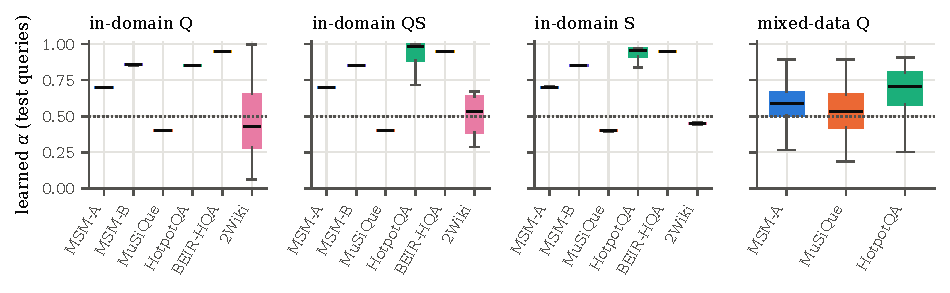
\includegraphics[width=\textwidth]{figures/gate_alpha.pdf}
  \caption{Distribution of the learned $\alpha$ over test queries (seed-averaged; min--max). In-domain
  gates collapse onto their initialisation $\alpha_0$ except on HotpotQA (\gate{QS}, \gate{S}) and 2Wiki
  (\gate{Q}, \gate{QS}); the gate trained on mixed data (\S\ref{sec:transfer}) spreads $\alpha$ and
  places MuSiQue lowest.}
  \label{fig:gate}
\end{figure*}

Table~\ref{tab:grid} compares every gate with the best fixed $\alpha$ under the same normaliser on all
six test sets. Of 76 comparisons, 11 are significantly positive and 13 significantly negative, and the
positives are of two kinds. (i) Gains of at most 0.05 points (MS MARCO under min--max and z-score),
which are statistically detectable on 7k queries but practically null. (ii) Larger gains where the
fixed baseline of that normaliser is weak: under rank normalisation the gates add up to +1.37 on MuSiQue
and +0.41 on 2Wiki, but recover only part of the gap to min--max (MuSiQue: rank 69.58 $\to$ 70.96 vs.\
min--max fixed 71.28). The one gain that yields a best-in-dataset system is z-score \gate{Q} on
BEIR-HotpotQA (+0.18, 72.87). There is no sign that gains are larger on multi-hop data (H2,
Table~\ref{tab:hyp}).

\paragraph{Why the gates do not adapt.}
Table~\ref{tab:gate} and Figure~\ref{fig:gate} show what the gates learn. On MS MARCO, MuSiQue and
BEIR-HotpotQA, the standard deviation of the learned $\alpha$ across test queries is at most 0.002:
in 100\% of these runs the best validation epoch is the initialisation, so early stopping returns the
fixed baseline. Training does move the gate (on MuSiQue validation nDCG@10 drops from 78.3 to 75.3
after one epoch for \gate{Q}), but every move hurts validation, so it is undone. On HotpotQA
(\gate{QS}, \gate{S}) and 2Wiki (\gate{Q}, \gate{QS}) the gates do adapt (sd 0.08--0.24), yet their
gains stay within noise. The 2Wiki \gate{Q} gate learns the right direction (mean $\alpha$ 0.72 for
comparison, 0.30 for inference, 0.35 for bridge-comparison questions, cf.\ Table~\ref{tab:bucket}) and
gains significantly on bridge-comparison questions (+0.16, $p<0.001$), but loses on inference
questions ($-0.23$, $p=0.016$), which cancels the gain overall. On HotpotQA the \gate{QS} gate puts
\emph{higher} $\alpha$ on comparison than on bridge questions (0.90 vs.\ 0.88), the opposite of what
their optima ask for. Three factors explain this: the per-query signal is weak (many queries are
indifferent to $\alpha$: between 14\% (MuSiQue) and 59\% (MS MARCO B) of test queries have the same
nDCG@10 for every $\alpha$);
the listwise training loss on fusion-train does not track validation nDCG@10; and the
train/validation shift of \S\ref{sec:dataset} makes the validation set disagree with the test set.
Explicit complexity features (\gate{QS+C}) and removing the regulariser ($\lambda{=}0$, appendix
tables) change nothing.

\begin{table*}[t]
\centering\small\setlength{\tabcolsep}{4pt}
\begin{tabular}{llrp{7.2cm}rr}
\toprule
Data & Buckets & $\alpha_0$ & Per-bucket $\alpha$ (chosen on val) & $\Delta$ & 95\% CI \\
\midrule
MSM-A & length & 0.70 & {\scriptsize long ($\ge$8 w) 0.75; medium (5--7 w) 0.45; short ($\le$4 w) 0.70} & -0.69$^{\triangledown}$ & [-0.87, -0.52] \\
MSM-A & wh-word & 0.70 & {\scriptsize how 0.85; other 0.55; what 0.45; when 0.85; where 0.85; who 0.85; why 0.85} & -0.79$^{\triangledown}$ & [-1.01, -0.57] \\
MSM-B & length & 0.85 & {\scriptsize long ($\ge$8 w) 1.00; medium (5--7 w) 0.85; short ($\le$4 w) 0.75} & -0.03 & [-0.30, +0.24] \\
MuSiQue & length & 0.40 & {\scriptsize long ($\ge$8 w) 0.40; medium (5--7 w) 0.15} & -0.01 & [-0.02, +0.00] \\
MuSiQue & hops (gold) & 0.40 & {\scriptsize 2-hop 0.40; 3-hop 0.40; 4-hop 0.25} & -0.03 & [-0.14, +0.08] \\
HotpotQA & length & 0.85 & {\scriptsize long ($\ge$8 w) 0.80; medium (5--7 w) 0.85} & -0.03 & [-0.09, +0.02] \\
HotpotQA & type (gold) & 0.85 & {\scriptsize bridge 1.00; comparison 0.40} & +0.14$^{\blacktriangle}$ & [+0.02, +0.25] \\
BEIR-HQA & length & 0.95 & {\scriptsize long ($\ge$8 w) 0.95; medium (5--7 w) 1.00} & -0.00 & [-0.01, +0.00] \\
BEIR-HQA & type (gold) & 0.95 & {\scriptsize bridge 1.00; comparison 0.65} & +0.42$^{\blacktriangle}$ & [+0.30, +0.53] \\
2Wiki & length & 0.45 & {\scriptsize long ($\ge$8 w) 0.45; medium (5--7 w) 0.20} & +0.00 & [-0.02, +0.02] \\
2Wiki & type (gold) & 0.45 & {\scriptsize bridge-comp. 0.25; comparison 0.90; compositional 0.45; inference 0.25} & +0.07$^{\blacktriangle}$ & [+0.01, +0.12] \\
\bottomrule
\end{tabular}
\caption{Bucketed fixed $\alpha$: one $\alpha$ per bucket selected on val and applied on test, against the single global $\alpha_0$ (test $\Delta$nDCG@10 $\times$100, paired bootstrap). Length buckets are available at test time; gold hop/type labels are not, so those rows measure how much a type-aware $\alpha$ \emph{could} give (analysis only).}
\label{tab:bucketed}
\end{table*}


\paragraph{Coarse, type-aware weights.}
If gates fail to learn per-query structure, a coarser query-dependent $\alpha$ may still help.
Table~\ref{tab:bucketed} selects one $\alpha$ per bucket on validation and applies it on test. With
gold question types this is significantly better than the global $\alpha_0$ on HotpotQA (+0.14),
BEIR-HotpotQA (+0.42) and 2Wiki (+0.07); hop-count buckets on MuSiQue do not help ($-0.03$, n.s.)
because of the validation/test shift. Query-length buckets, which are available at test time, never
help and hurt on MS MARCO A ($-0.69$), again because validation is unrepresentative there. So a
query-dependent $\alpha$ can beat a fixed one when the dependence follows a reliable, coarse property
of the query, but the gain is small and depends on labels not available at test time.

% ---------------------------------------------------------------------
\subsection{Pre-registered tests}
\begin{table*}[t]
\centering\small\setlength{\tabcolsep}{3.5pt}
\begin{tabular}{llllrlrcl}
\toprule
Hyp. & Dataset & Gate & Statistic & Value & 95\% CI & $p_{\text{Holm}}$ & Pred. & Verdict \\
\midrule
H1 & MuSiQue & best=Q & Spearman($\alpha$, hops) & +0.107 & [+0.067, +0.147] & 0.001 & <0 & contradicted \\
H2 & MuSiQue & best=Q & gain $-$ gain$_{\text{MSM}}$ & -0.004 & [-0.025, +0.017] & 1.000 & >0 & inconclusive \\
H3 & MuSiQue & oracle & headroom $-$ headroom$_{\text{MSM}}$ & +2.435 & [+1.942, +2.932] & 0.001 & >0 & supported \\
H1 & HotpotQA & best=QS & $\bar\alpha_{\text{bridge}}-\bar\alpha_{\text{comp.}}$ & -0.026 & [-0.037, -0.016] & 0.001 & <0 & supported \\
H2 & HotpotQA & best=QS & gain $-$ gain$_{\text{MSM}}$ & +0.011 & [-0.095, +0.117] & 1.000 & >0 & inconclusive \\
H3 & HotpotQA & oracle & headroom $-$ headroom$_{\text{MSM}}$ & -2.036 & [-2.365, -1.710] & 0.001 & >0 & contradicted \\
H1 & BEIR-HotpotQA & best=Q & $\bar\alpha_{\text{bridge}}-\bar\alpha_{\text{comp.}}$ & +0.000 & [+0.000, +0.000] & 0.001 & <0 & contradicted \\
H2 & BEIR-HotpotQA & best=Q & gain $-$ gain$_{\text{MSM}}$ & -0.005 & [-0.025, +0.016] & 1.000 & >0 & inconclusive \\
H3 & BEIR-HotpotQA & oracle & headroom $-$ headroom$_{\text{MSM}}$ & -2.078 & [-2.427, -1.739] & 0.001 & >0 & contradicted \\
\bottomrule
\end{tabular}
\caption{Pre-registered primary tests (written before any multi-hop run; Holm over the nine tests). H1 uses the best (on val) gate; H2/H3 values are nDCG@10 $\times$100. H1 verdicts on MuSiQue and BEIR are computed on gates whose $\alpha$ varies by less than $10^{-3}$ across queries (Table~\ref{tab:gate}), so their sign is not interpretable.}
\label{tab:hyp}
\end{table*}


Table~\ref{tab:hyp} reports the nine primary tests exactly as pre-registered. H3 is supported only on
MuSiQue: its oracle headroom (7.4 points) exceeds MS MARCO's (5.0) by 2.4 points, whereas HotpotQA and
BEIR-HotpotQA have \emph{less} headroom than MS MARCO (3.0 and 2.9 points). H2 is inconclusive everywhere.
H1 is ``supported'' on HotpotQA ($\bar\alpha_\text{bridge}-\bar\alpha_\text{comp.}=-0.026$) and
``contradicted'' on MuSiQue and BEIR-HotpotQA; the latter two verdicts are artefacts, since those gates'
$\alpha$ varies by less than $10^{-3}$, and the HotpotQA verdict concerns a gate whose $\alpha$ moves in
the direction opposite to its own nDCG optimum (\S\ref{sec:gates}). We therefore base our conclusions on
the bucket optima (\S\ref{sec:query}), which do not depend on whether a gate learned anything.

% ---------------------------------------------------------------------
\subsection{Graph controls (H4)}
\begin{table*}[t]
\centering\small\setlength{\tabcolsep}{4pt}
\begin{tabular}{llrrrrrrr}
\toprule
Dataset & Graph & Degree & Gold pairs & GAT & $\alpha_0$ & Fixed & $\Delta$ adaptive & Headroom \\
 & & & linked (\%) & nDCG@10 & & nDCG@10 & (best gate) & (oracle) \\
\midrule
MuSiQue & none (self-loops) & 0.00 & 0 & 67.7 & 0.35 & 71.75 & -0.03 & 7.7 \\
 & random (same degrees) & 2.78 & 14 & 67.0 & 0.50 & 71.89 & -0.03 & 6.6 \\
 & kNN emb. (default) & 2.78 & 27 & 66.8 & 0.40 & 71.28 & +0.00 & 7.4 \\
 & title link & 0.81 & 19 & 68.0 & 0.35 & 71.97 & +0.00 & 7.6 \\
 & kNN $\cup$ title & 3.20 & 36 & 67.0 & 0.40 & 71.40 & +0.00 & 7.4 \\
\midrule
HotpotQA & none (self-loops) & 0.00 & 0 & 84.6 & 0.85 & 89.98 & +0.02 & 3.0 \\
 & random (same degrees) & 2.78 & 31 & 83.7 & 0.90 & 89.89 & -0.02 & 2.8 \\
 & kNN emb. (default) & 2.78 & 48 & 84.1 & 0.85 & 89.87 & +0.02 & 3.0 \\
 & title link & 0.98 & 68 & 87.4 & 0.65 & 90.52 & +0.05 & 3.5 \\
 & kNN $\cup$ title & 3.18 & 80 & 85.5 & 0.65 & 89.97 & +0.18$^{\blacktriangle}$ & 3.4 \\
\bottomrule
\end{tabular}
\caption{Graph controls (H4, exploratory): a GAT retrained per graph type, everything else fixed. Degree excludes self-loops; ``gold pairs linked'' = share of supporting-paragraph pairs joined by an edge (test). nDCG@10 and $\Delta$ are $\times$100 on test; $\Delta$ = best gate (on val) $-$ best fixed $\alpha$, $^{\blacktriangle}$ $p<0.05$.}
\label{tab:graph}
\end{table*}


Table~\ref{tab:graph} retrains the GAT on five graph types. On MuSiQue the graph structure barely
matters: GAT-only nDCG@10 is 67.7 with no edges at all, 66.8 with the default $k$-NN graph and 68.0 with
title links, and the headroom and the (null) adaptive gains are the same for every graph, including
random and empty ones. The MuSiQue effects of \S\ref{sec:query} therefore come from the GAT's
query--passage representation (trained in-domain with a listwise loss), not from message passing.
On HotpotQA, edges matter: title links connect 68\% of the gold pairs (vs.\ 48\% for $k$-NN, 31\% for
random), raise GAT-only by 3.3 points, lower $\alpha_0$ to 0.65 and give the best HotpotQA system
(90.52). The only significant adaptive gain in this table is on the hybrid graph (+0.18), where 80\% of
gold pairs are linked. On MS MARCO the $k$-NN graph is within 0.1 points of the empty and random graphs
(Appendix~\ref{app:controls}).

% ---------------------------------------------------------------------
\subsection{Transfer and mixed training}
\label{sec:transfer}
\begin{table*}[t]
\centering\small\setlength{\tabcolsep}{4pt}
\resizebox{\textwidth}{!}{%
\begin{tabular}{lllrrrrrrr}
\toprule
 & & & \multicolumn{4}{c}{Transferred gate, test nDCG@10} & In-domain & & \textsc{Q} gate \\
\cmidrule(lr){4-7}
Setting & Train & Test & fixed & \textsc{Q} & \textsc{QS} & \textsc{S} & fixed & $\alpha_0$ & $\bar\alpha$ (sd) \\
\midrule
leave-one-out & MSM+HQA & MuSiQue & 71.99 & 71.93 & 71.98 & 72.00 & 71.28 & 0.70 & 0.73 (0.02) \\
mixed & MSM+MuSiQue+HQA & MuSiQue & 71.98 & 71.77 & 71.81 & 71.79 & 71.28 & 0.55 & 0.54 (0.16) \\
zero-shot & MSM & BEIR-HotpotQA & 71.45 & 71.45 & 71.45 & 71.46 & 72.63 & 0.70 & 0.70 (0.00) \\
zero-shot & MSM & HotpotQA & 89.24 & 89.24 & 89.25 & 89.20 & 89.89 & 0.70 & 0.70 (0.00) \\
zero-shot & MSM & 2Wiki & 90.99 & 90.99 & 90.99 & 90.99 & 91.75 & 0.70 & 0.70 (0.00) \\
\bottomrule
\end{tabular}}
\caption{Transfer and mixed training of the gate (E4, min--max, $\times$100, 5 seeds). Zero-shot uses the frozen MS MARCO GAT for $s_{ctx}$; mixed and leave-one-out use each dataset's own GAT. $\alpha_0$ is the fixed $\alpha$ the gate starts from (selected on the training sources' val).}
\label{tab:transfer}
\end{table*}


Table~\ref{tab:transfer} tests whether a gate learns to separate simple from complex queries when it
sees both. A zero-shot gate trained on MS MARCO stays at its initialisation (sd 0.00); its MuSiQue
score is higher than the in-domain gate's only because MS MARCO's $\alpha_0=0.70$ happens to be closer
to MuSiQue's test optimum (0.65) than MuSiQue's own validation-selected 0.40. A single \gate{Q} gate
trained on MS MARCO, MuSiQue and HotpotQA together does adapt (sd 0.12--0.16) and orders the datasets as
the hypothesis predicts: mean $\alpha$ 0.54 on MuSiQue, 0.59 on MS MARCO and 0.68 on HotpotQA. It still
loses to the in-domain fixed weights on MS MARCO ($-0.60$) and HotpotQA ($-0.45$), so the gate captures
the coarse dataset-level difference but not enough of it to pay off.

\begin{table*}[t]
\centering\small\setlength{\tabcolsep}{3pt}
\begin{tabular}{p{4.2cm}p{9.0cm}l}
\toprule
Claim & Evidence & Verdict \\
\midrule
C1: $\alpha>0.5$ single-hop & MS MARCO 0.70--0.95 & supported \\
C1: $\alpha<0.5$ multi-hop & 2Wiki 0.45; MuSiQue 0.40 (val), 0.65 (test); HotpotQA 0.85--0.95 & partly \\
C2: $\alpha$ falls with complexity & MuSiQue 0.80/0.55/0.40; 2Wiki comp.\ 0.65 vs.\ others 0.20--0.50; HotpotQA reversed & partly \\
C3: adaptive $>$ fixed & 11/76 cells better, 13 worse; gains $\le$0.04 under primary norm.; oracle 2.3--7.4 & not supported \\
C3: larger gain on multi-hop & H2 inconclusive on all datasets & not supported \\
\bottomrule
\end{tabular}
\caption{Verdict on the hypothesis.}
\label{tab:verdict}
\end{table*}

\FloatBarrier
% =====================================================================
\section{Discussion}
\label{sec:discussion}



Table~\ref{tab:verdict} summarises the evidence. The intuition behind the hypothesis is right in one
important sense: the fusion weight that a query \emph{should} get is not constant, it differs by up
to 0.65 between question types of one dataset (2Wiki validation: 0.90 vs.\ 0.25), and on the hardest multi-hop questions it moves
to the contextual side. What the hypothesis gets wrong is the mechanism and the method. The mechanism
is relative reliability: complexity lowers $\alpha^*$ only where it makes the cross-encoder, which reads
each passage in isolation, worse than the graph-refined score, as on 4-hop MuSiQue and
bridge-comparison 2Wiki questions; where single-paragraph matching still works (HotpotQA bridge questions)
the cross-encoder keeps the weight. The method fails because a gate must infer, from one query embedding
or a dozen score statistics, a property that changes the optimal weight for only a minority of queries,
and early stopping on a validation set that is itself shifted rejects every move.

Two practical lessons follow. First, the fixed weight should be selected on validation data drawn
from the test distribution: on MS MARCO A and MuSiQue the test-optimal fixed $\alpha$ is 0.25 above the
validation choice and would add 0.54 and 0.79 nDCG@10 points, more than any gate. Second,
improving the contextual signal itself (title links on HotpotQA: +0.65 points for fixed fusion) is
worth more than making its weight adaptive.

% =====================================================================
\section{Conclusion}
\label{sec:conclusion}
We tested whether the weight between a cross-encoder and a graph-contextual score should depend on
query complexity. The optimal weight does vary: it is above 0.5 on MS MARCO, below 0.5 on
2WikiMultiHopQA, and it falls with the hop count on MuSiQue. This variation is explained by the relative
reliability of the two scores ($\rho=0.79$ across buckets) rather than by complexity as such. Learned
query-dependent gates, however, do not exploit it. They collapse to the fixed weight and gain at most 0.04
nDCG@10 points over it under the primary normaliser, although an oracle shows 2.3--7.4 points of headroom.
A coarse weight per question type is the only query-dependent scheme that helps, and only modestly.

% =====================================================================
\section*{Limitations}
All models are small MiniLM checkpoints trained on MS MARCO and are never fine-tuned on the multi-hop
data; a cross-encoder trained on multi-hop data would shift every optimum towards $\alpha=1$. Three of the
multi-hop settings are closed pools in which the gold paragraphs are always present, so they test
reranking, not retrieval. The graphs are per-query candidate graphs; ReGAT-BERT's original structural
edges cannot be built on MS MARCO, and our results concern this adaptation, not a replication. The
validation sets of MS MARCO A and the closed-pool datasets are carved from training questions, which
causes the validation/test shift we report. Complexity labels on MS MARCO are heuristic proxies. Bucket
optima are computed on test data for analysis; they are never used to select a reported system, but the
type-aware results in Table~\ref{tab:bucketed} use gold labels unavailable at test time. Significance marks
in the ablation grid are uncorrected; only the nine primary tests are Holm-corrected.

\section*{Ethics Statement}
We use public research datasets under their licences and release no new data. The work does not
involve human subjects or personal data beyond what these benchmarks already contain.

\bibliography{references}

% =====================================================================
\clearpage
\appendix

\section{Full results}
\label{app:full}
Tables~\ref{tab:full_A}--\ref{tab:full_twowiki} report nDCG, MRR, Precision and Recall at
$k\in\{1,3,5,10,50\}$ and MAP on every test set for the reference rows, all gates (with $\lambda=0.01$
and $\lambda=0$), the BCE loss ablation and the oracle. Precision@$k$ divides by $k$; on closed pools the
pool size bounds Recall@50 and Precision@50. Table~\ref{tab:trec} gives the out-of-distribution TREC DL
2019/2020 results \citep{craswell2020trec,craswell2021trec} for MS MARCO.

\begin{table*}[t]
\centering
\resizebox{\textwidth}{!}{%
\begin{tabular}{lrrrrrrrrrrrrrrrrrrrrr}
\toprule
 & \multicolumn{5}{c}{nDCG@$k$} & \multicolumn{5}{c}{MRR@$k$} & \multicolumn{5}{c}{P@$k$} & \multicolumn{5}{c}{R@$k$} & \\
\cmidrule(lr){2-6} \cmidrule(lr){7-11} \cmidrule(lr){12-16} \cmidrule(lr){17-21}
 & 1 & 3 & 5 & 10 & 50 & 1 & 3 & 5 & 10 & 50 & 1 & 3 & 5 & 10 & 50 & 1 & 3 & 5 & 10 & 50 & MAP \\
\midrule
BM25 (first stage / in-pool) & 10.5 & 17.0 & 19.7 & 22.8 & 27.4 & 10.5 & 15.6 & 17.1 & 18.4 & 19.4 & 10.5 & 7.5 & 5.9 & 3.9 & 1.2 & 10.2 & 21.7 & 28.5 & 37.9 & 58.1 & 19.2 \\
SBERT ($s_{bi}$) & 20.4 & 29.3 & 32.4 & 35.3 & 38.2 & 20.4 & 27.5 & 29.2 & 30.4 & 31.1 & 20.4 & 12.3 & 9.0 & 5.4 & 1.4 & 19.8 & 35.7 & 43.2 & 52.0 & 64.4 & 30.6 \\
CE only ($\alpha{=}1$) & 25.5 & 35.6 & 38.8 & 41.3 & 43.1 & 25.5 & 33.6 & 35.4 & 36.4 & 36.8 & 25.5 & 14.8 & 10.5 & 6.1 & 1.4 & 24.7 & 42.9 & 50.5 & 58.2 & 65.4 & 36.2 \\
GAT only ($\alpha{=}0$) & 20.4 & 29.2 & 32.4 & 35.4 & 38.2 & 20.4 & 27.4 & 29.2 & 30.4 & 31.1 & 20.4 & 12.3 & 9.0 & 5.5 & 1.4 & 19.8 & 35.6 & 43.3 & 52.4 & 64.5 & 30.6 \\
\midrule
ReGAT-BERT-style ($a,b$; BCE) & 23.9 & 33.8 & 37.1 & 39.8 & 41.8 & 23.9 & 31.8 & 33.6 & 34.7 & 35.2 & 23.9 & 14.2 & 10.2 & 6.0 & 1.4 & 23.2 & 41.0 & 48.8 & 57.1 & 65.4 & 34.6 \\
Fixed $\alpha$ (grid on val) & 25.0 & 35.1 & 38.4 & 40.9 & 42.7 & 25.0 & 33.0 & 34.8 & 35.9 & 36.3 & 25.0 & 14.7 & 10.5 & 6.0 & 1.4 & 24.3 & 42.4 & 50.3 & 57.9 & 65.4 & 35.7 \\
Fixed $\alpha$ (learned) & 25.0 & 35.1 & 38.4 & 40.9 & 42.7 & 25.0 & 33.0 & 34.8 & 35.9 & 36.3 & 25.0 & 14.7 & 10.5 & 6.0 & 1.4 & 24.3 & 42.4 & 50.3 & 57.9 & 65.4 & 35.7 \\
\midrule
Adaptive $\alpha(q)$ \textsc{Q} & 25.0 & 35.1 & 38.4 & 40.9 & 42.7 & 25.0 & 33.0 & 34.8 & 35.9 & 36.3 & 25.0 & 14.7 & 10.5 & 6.0 & 1.4 & 24.3 & 42.4 & 50.3 & 57.9 & 65.4 & 35.7 \\
Adaptive $\alpha(q,s)$ \textsc{QS} & 24.9 & 35.1 & 38.4 & 40.9 & 42.7 & 24.9 & 33.0 & 34.8 & 35.9 & 36.3 & 24.9 & 14.7 & 10.5 & 6.0 & 1.4 & 24.3 & 42.4 & 50.3 & 57.9 & 65.4 & 35.7 \\
Adaptive $\alpha(s)$ \textsc{S} & 25.0 & 35.1 & 38.4 & 40.9 & 42.7 & 25.0 & 33.1 & 34.8 & 35.9 & 36.3 & 25.0 & 14.7 & 10.5 & 6.0 & 1.4 & 24.3 & 42.4 & 50.2 & 57.9 & 65.4 & 35.7 \\
\textsc{Q}, $\lambda=0$ & 25.0 & 35.1 & 38.4 & 40.9 & 42.7 & 25.0 & 33.0 & 34.8 & 35.9 & 36.3 & 25.0 & 14.7 & 10.5 & 6.0 & 1.4 & 24.3 & 42.4 & 50.3 & 57.9 & 65.4 & 35.7 \\
\textsc{QS}, $\lambda=0$ & 24.9 & 35.1 & 38.4 & 40.9 & 42.7 & 24.9 & 33.0 & 34.8 & 35.9 & 36.3 & 24.9 & 14.7 & 10.5 & 6.0 & 1.4 & 24.3 & 42.4 & 50.3 & 57.9 & 65.4 & 35.7 \\
\textsc{S}, $\lambda=0$ & 25.0 & 35.1 & 38.4 & 40.9 & 42.7 & 25.0 & 33.1 & 34.8 & 35.9 & 36.3 & 25.0 & 14.7 & 10.5 & 6.0 & 1.4 & 24.3 & 42.4 & 50.2 & 57.9 & 65.4 & 35.7 \\
Fixed $\alpha$, BCE loss (minmax) & 25.0 & 35.1 & 38.4 & 40.9 & 42.7 & 25.0 & 33.0 & 34.8 & 35.9 & 36.3 & 25.0 & 14.7 & 10.5 & 6.0 & 1.4 & 24.3 & 42.4 & 50.3 & 57.9 & 65.4 & 35.7 \\
\textsc{QS}, BCE loss (minmax) & 24.9 & 35.1 & 38.4 & 40.9 & 42.7 & 24.9 & 33.0 & 34.8 & 35.9 & 36.3 & 24.9 & 14.7 & 10.5 & 6.0 & 1.4 & 24.3 & 42.4 & 50.3 & 57.9 & 65.4 & 35.7 \\
\midrule
\textit{Oracle per-query $\alpha$ (bound)} & 32.1 & 41.3 & 43.9 & 45.9 & 47.1 & 32.1 & 39.6 & 41.0 & 41.8 & 42.1 & 32.1 & 16.6 & 11.3 & 6.3 & 1.4 & 31.2 & 47.9 & 54.1 & 60.1 & 65.4 & 41.4 \\
\bottomrule
\end{tabular}}
\caption{MS MARCO (A): all test metrics ($\times$100, mean over seeds), min--max normaliser unless stated.}
\label{tab:full_A}
\end{table*}

\begin{table*}[t]
\centering
\resizebox{\textwidth}{!}{%
\begin{tabular}{lrrrrrrrrrrrrrrrrrrrrr}
\toprule
 & \multicolumn{5}{c}{nDCG@$k$} & \multicolumn{5}{c}{MRR@$k$} & \multicolumn{5}{c}{P@$k$} & \multicolumn{5}{c}{R@$k$} & \\
\cmidrule(lr){2-6} \cmidrule(lr){7-11} \cmidrule(lr){12-16} \cmidrule(lr){17-21}
 & 1 & 3 & 5 & 10 & 50 & 1 & 3 & 5 & 10 & 50 & 1 & 3 & 5 & 10 & 50 & 1 & 3 & 5 & 10 & 50 & MAP \\
\midrule
BM25 (first stage / in-pool) & 10.3 & 17.4 & 19.9 & 23.0 & 27.6 & 10.3 & 15.8 & 17.2 & 18.5 & 19.6 & 10.3 & 7.7 & 5.9 & 3.9 & 1.2 & 10.1 & 22.5 & 28.7 & 37.9 & 58.1 & 19.4 \\
SBERT ($s_{bi}$) & 20.7 & 30.2 & 33.1 & 35.7 & 38.6 & 20.7 & 28.1 & 29.7 & 30.9 & 31.5 & 20.7 & 12.7 & 9.1 & 5.4 & 1.4 & 20.3 & 37.0 & 44.0 & 51.9 & 64.2 & 31.1 \\
CE only ($\alpha{=}1$) & 25.4 & 36.2 & 39.1 & 41.5 & 43.3 & 25.4 & 33.9 & 35.6 & 36.6 & 37.0 & 25.4 & 15.2 & 10.6 & 6.1 & 1.4 & 24.8 & 43.9 & 50.9 & 58.1 & 65.3 & 36.5 \\
GAT only ($\alpha{=}0$) & 19.9 & 30.1 & 33.0 & 35.7 & 38.4 & 19.9 & 27.9 & 29.4 & 30.6 & 31.2 & 19.9 & 12.9 & 9.2 & 5.5 & 1.4 & 19.5 & 37.6 & 44.6 & 52.7 & 64.6 & 30.7 \\
\midrule
ReGAT-BERT-style ($a,b$; BCE) & 24.5 & 34.3 & 37.9 & 40.2 & 42.2 & 24.5 & 32.2 & 34.2 & 35.2 & 35.7 & 24.5 & 14.3 & 10.4 & 6.0 & 1.4 & 23.9 & 41.5 & 50.0 & 57.1 & 65.2 & 35.2 \\
Fixed $\alpha$ (grid on val) & 26.0 & 36.3 & 39.3 & 41.7 & 43.5 & 26.0 & 34.2 & 35.9 & 36.8 & 37.3 & 26.0 & 15.2 & 10.6 & 6.1 & 1.4 & 25.4 & 43.8 & 50.9 & 58.0 & 65.3 & 36.7 \\
Fixed $\alpha$ (learned) & 26.0 & 36.3 & 39.3 & 41.7 & 43.5 & 26.0 & 34.2 & 35.9 & 36.8 & 37.3 & 26.0 & 15.2 & 10.6 & 6.1 & 1.4 & 25.4 & 43.8 & 50.9 & 58.0 & 65.3 & 36.7 \\
\midrule
Adaptive $\alpha(q)$ \textsc{Q} & 26.0 & 36.3 & 39.3 & 41.7 & 43.5 & 26.0 & 34.2 & 35.8 & 36.8 & 37.2 & 26.0 & 15.2 & 10.6 & 6.1 & 1.4 & 25.3 & 43.8 & 50.9 & 58.1 & 65.3 & 36.7 \\
Adaptive $\alpha(q,s)$ \textsc{QS} & 26.0 & 36.3 & 39.4 & 41.7 & 43.5 & 26.0 & 34.2 & 35.9 & 36.8 & 37.3 & 26.0 & 15.1 & 10.6 & 6.1 & 1.4 & 25.4 & 43.8 & 50.9 & 58.0 & 65.3 & 36.7 \\
Adaptive $\alpha(s)$ \textsc{S} & 26.1 & 36.3 & 39.4 & 41.7 & 43.5 & 26.1 & 34.2 & 35.9 & 36.9 & 37.3 & 26.1 & 15.1 & 10.6 & 6.1 & 1.4 & 25.4 & 43.8 & 50.9 & 58.0 & 65.3 & 36.7 \\
\textsc{Q}, $\lambda=0$ & 26.0 & 36.3 & 39.3 & 41.7 & 43.5 & 26.0 & 34.2 & 35.8 & 36.8 & 37.2 & 26.0 & 15.2 & 10.6 & 6.1 & 1.4 & 25.3 & 43.8 & 50.9 & 58.1 & 65.3 & 36.7 \\
\textsc{QS}, $\lambda=0$ & 26.0 & 36.3 & 39.4 & 41.7 & 43.5 & 26.0 & 34.2 & 35.9 & 36.8 & 37.3 & 26.0 & 15.1 & 10.6 & 6.1 & 1.4 & 25.4 & 43.8 & 50.9 & 58.0 & 65.3 & 36.7 \\
\textsc{S}, $\lambda=0$ & 26.1 & 36.3 & 39.4 & 41.7 & 43.5 & 26.1 & 34.2 & 35.9 & 36.9 & 37.3 & 26.1 & 15.1 & 10.6 & 6.1 & 1.4 & 25.4 & 43.8 & 50.9 & 58.0 & 65.3 & 36.7 \\
Fixed $\alpha$, BCE loss (zscore) & 25.8 & 36.4 & 39.3 & 41.5 & 43.4 & 25.8 & 34.1 & 35.7 & 36.7 & 37.1 & 25.8 & 15.2 & 10.6 & 6.0 & 1.4 & 25.2 & 44.0 & 51.0 & 57.8 & 65.3 & 36.6 \\
\textsc{QS}, BCE loss (zscore) & 25.9 & 36.3 & 39.3 & 41.6 & 43.4 & 25.9 & 34.1 & 35.8 & 36.7 & 37.1 & 25.9 & 15.2 & 10.6 & 6.0 & 1.4 & 25.3 & 43.9 & 51.0 & 57.8 & 65.3 & 36.6 \\
\midrule
\textit{Oracle per-query $\alpha$ (bound)} & 32.0 & 41.8 & 44.3 & 46.0 & 47.3 & 32.0 & 39.9 & 41.2 & 41.9 & 42.2 & 32.0 & 16.9 & 11.5 & 6.3 & 1.4 & 31.1 & 48.8 & 54.9 & 60.1 & 65.4 & 41.5 \\
\bottomrule
\end{tabular}}
\caption{MS MARCO (B): all test metrics ($\times$100, mean over seeds), min--max normaliser unless stated.}
\label{tab:full_B}
\end{table*}

\begin{table*}[t]
\centering
\resizebox{\textwidth}{!}{%
\begin{tabular}{lrrrrrrrrrrrrrrrrrrrrr}
\toprule
 & \multicolumn{5}{c}{nDCG@$k$} & \multicolumn{5}{c}{MRR@$k$} & \multicolumn{5}{c}{P@$k$} & \multicolumn{5}{c}{R@$k$} & \\
\cmidrule(lr){2-6} \cmidrule(lr){7-11} \cmidrule(lr){12-16} \cmidrule(lr){17-21}
 & 1 & 3 & 5 & 10 & 50 & 1 & 3 & 5 & 10 & 50 & 1 & 3 & 5 & 10 & 50 & 1 & 3 & 5 & 10 & 50 & MAP \\
\midrule
BM25 (first stage / in-pool) & 66.9 & 48.6 & 50.9 & 55.1 & 68.6 & 66.9 & 73.7 & 74.8 & 75.7 & 76.1 & 66.9 & 35.5 & 24.7 & 14.9 & 5.3 & 27.3 & 42.3 & 48.6 & 58.2 & 100.0 & 48.9 \\
SBERT ($s_{bi}$) & 72.6 & 54.3 & 59.4 & 67.1 & 74.8 & 72.6 & 80.0 & 81.4 & 81.8 & 81.9 & 72.6 & 40.7 & 30.9 & 20.2 & 5.3 & 29.3 & 47.9 & 59.9 & 77.4 & 100.0 & 57.2 \\
CE only ($\alpha{=}1$) & 79.8 & 61.9 & 65.4 & 71.1 & 78.7 & 79.8 & 86.3 & 87.0 & 87.3 & 87.4 & 79.8 & 46.5 & 32.9 & 20.1 & 5.3 & 32.4 & 55.3 & 64.3 & 77.4 & 100.0 & 62.6 \\
GAT only ($\alpha{=}0$) & 72.4 & 53.9 & 58.9 & 66.8 & 74.7 & 72.4 & 79.5 & 80.9 & 81.5 & 81.6 & 72.4 & 40.2 & 30.6 & 20.2 & 5.3 & 29.3 & 47.4 & 59.1 & 77.1 & 100.0 & 57.1 \\
\midrule
ReGAT-BERT-style ($a,b$; BCE) & 79.8 & 61.7 & 65.4 & 71.7 & 79.0 & 79.8 & 86.2 & 86.9 & 87.3 & 87.3 & 79.8 & 46.4 & 33.2 & 20.6 & 5.3 & 32.5 & 54.7 & 64.5 & 78.8 & 100.0 & 63.0 \\
Fixed $\alpha$ (grid on val) & 78.4 & 60.6 & 64.7 & 71.3 & 78.4 & 78.4 & 85.1 & 85.9 & 86.3 & 86.3 & 78.4 & 45.7 & 33.1 & 20.7 & 5.3 & 31.9 & 53.8 & 64.2 & 79.2 & 100.0 & 62.3 \\
Fixed $\alpha$ (learned) & 78.4 & 60.6 & 64.7 & 71.3 & 78.4 & 78.4 & 85.1 & 85.9 & 86.3 & 86.3 & 78.4 & 45.7 & 33.1 & 20.7 & 5.3 & 31.9 & 53.8 & 64.2 & 79.2 & 100.0 & 62.3 \\
\midrule
Adaptive $\alpha(q)$ \textsc{Q} & 78.4 & 60.6 & 64.7 & 71.3 & 78.4 & 78.4 & 85.1 & 85.9 & 86.3 & 86.3 & 78.4 & 45.7 & 33.1 & 20.7 & 5.3 & 31.9 & 53.8 & 64.2 & 79.2 & 100.0 & 62.3 \\
Adaptive $\alpha(q,s)$ \textsc{QS} & 78.3 & 60.6 & 64.7 & 71.3 & 78.4 & 78.3 & 85.1 & 85.9 & 86.3 & 86.3 & 78.3 & 45.7 & 33.1 & 20.7 & 5.3 & 31.9 & 53.8 & 64.2 & 79.2 & 100.0 & 62.3 \\
Adaptive $\alpha(s)$ \textsc{S} & 78.4 & 60.6 & 64.7 & 71.3 & 78.4 & 78.4 & 85.1 & 85.9 & 86.3 & 86.3 & 78.4 & 45.7 & 33.1 & 20.7 & 5.3 & 31.9 & 53.8 & 64.2 & 79.2 & 100.0 & 62.3 \\
Adaptive \textsc{QS+C} & 78.4 & 60.6 & 64.7 & 71.3 & 78.4 & 78.4 & 85.1 & 85.9 & 86.3 & 86.3 & 78.4 & 45.7 & 33.1 & 20.7 & 5.3 & 31.9 & 53.8 & 64.2 & 79.2 & 100.0 & 62.3 \\
\textsc{Q}, $\lambda=0$ & 78.4 & 60.6 & 64.7 & 71.3 & 78.4 & 78.4 & 85.1 & 85.9 & 86.3 & 86.3 & 78.4 & 45.7 & 33.1 & 20.7 & 5.3 & 31.9 & 53.8 & 64.2 & 79.2 & 100.0 & 62.3 \\
\textsc{QS}, $\lambda=0$ & 78.3 & 60.6 & 64.7 & 71.3 & 78.4 & 78.3 & 85.1 & 85.9 & 86.3 & 86.3 & 78.3 & 45.7 & 33.1 & 20.7 & 5.3 & 31.9 & 53.8 & 64.2 & 79.2 & 100.0 & 62.3 \\
\textsc{S}, $\lambda=0$ & 78.4 & 60.6 & 64.7 & 71.3 & 78.4 & 78.4 & 85.1 & 85.9 & 86.3 & 86.3 & 78.4 & 45.7 & 33.1 & 20.7 & 5.3 & 31.9 & 53.8 & 64.2 & 79.2 & 100.0 & 62.3 \\
Fixed $\alpha$, BCE loss (zscore) & 79.3 & 61.0 & 65.0 & 71.5 & 78.6 & 79.3 & 85.7 & 86.5 & 86.9 & 86.9 & 79.3 & 45.9 & 33.1 & 20.6 & 5.3 & 32.2 & 54.1 & 64.3 & 79.0 & 100.0 & 62.6 \\
\textsc{QS}, BCE loss (zscore) & 80.3 & 61.4 & 65.2 & 71.8 & 78.9 & 80.3 & 86.2 & 87.0 & 87.4 & 87.4 & 80.3 & 46.1 & 33.0 & 20.7 & 5.3 & 32.6 & 54.5 & 64.2 & 79.3 & 100.0 & 62.9 \\
\midrule
\textit{Oracle per-query $\alpha$ (bound)} & 87.9 & 68.5 & 72.0 & 78.7 & 83.5 & 87.9 & 91.9 & 92.3 & 92.5 & 92.5 & 87.9 & 51.8 & 36.4 & 22.5 & 5.3 & 35.6 & 61.1 & 70.7 & 85.8 & 100.0 & 69.7 \\
\bottomrule
\end{tabular}}
\caption{MuSiQue: all test metrics ($\times$100, mean over seeds), min--max normaliser unless stated. Closed pools: every gold passage is in the pool, so R@50 $=1$ and P@50 = \#gold/50 for all rows (also R@10 $=1$ when $K=10$).}
\label{tab:full_musique}
\end{table*}

\begin{table*}[t]
\centering
\resizebox{\textwidth}{!}{%
\begin{tabular}{lrrrrrrrrrrrrrrrrrrrrr}
\toprule
 & \multicolumn{5}{c}{nDCG@$k$} & \multicolumn{5}{c}{MRR@$k$} & \multicolumn{5}{c}{P@$k$} & \multicolumn{5}{c}{R@$k$} & \\
\cmidrule(lr){2-6} \cmidrule(lr){7-11} \cmidrule(lr){12-16} \cmidrule(lr){17-21}
 & 1 & 3 & 5 & 10 & 50 & 1 & 3 & 5 & 10 & 50 & 1 & 3 & 5 & 10 & 50 & 1 & 3 & 5 & 10 & 50 & MAP \\
\midrule
BM25 (first stage / in-pool) & 81.2 & 67.6 & 71.9 & 81.7 & 81.7 & 81.2 & 86.6 & 87.4 & 87.9 & 87.9 & 81.2 & 43.5 & 29.4 & 20.0 & 4.0 & 40.6 & 65.2 & 73.6 & 100.0 & 100.0 & 69.3 \\
SBERT ($s_{bi}$) & 80.1 & 69.2 & 74.7 & 82.9 & 82.9 & 80.1 & 85.8 & 86.7 & 87.2 & 87.2 & 80.1 & 45.2 & 31.5 & 20.0 & 4.0 & 40.0 & 67.8 & 78.8 & 100.0 & 100.0 & 71.7 \\
CE only ($\alpha{=}1$) & 92.2 & 81.0 & 84.7 & 89.8 & 89.8 & 92.2 & 95.1 & 95.3 & 95.4 & 95.4 & 92.2 & 52.9 & 34.7 & 20.0 & 4.0 & 46.1 & 79.4 & 86.7 & 100.0 & 100.0 & 81.8 \\
GAT only ($\alpha{=}0$) & 81.7 & 71.1 & 76.7 & 84.1 & 84.1 & 81.7 & 87.2 & 88.0 & 88.4 & 88.4 & 81.7 & 46.6 & 32.5 & 20.0 & 4.0 & 40.8 & 69.9 & 81.1 & 100.0 & 100.0 & 73.5 \\
\midrule
ReGAT-BERT-style ($a,b$; BCE) & 92.1 & 81.1 & 84.8 & 89.9 & 89.9 & 92.1 & 95.0 & 95.3 & 95.3 & 95.3 & 92.1 & 52.9 & 34.7 & 20.0 & 4.0 & 46.1 & 79.4 & 86.7 & 100.0 & 100.0 & 81.9 \\
Fixed $\alpha$ (grid on val) & 92.0 & 81.1 & 84.8 & 89.9 & 89.9 & 92.0 & 95.0 & 95.2 & 95.3 & 95.3 & 92.0 & 53.0 & 34.7 & 20.0 & 4.0 & 46.0 & 79.5 & 86.8 & 100.0 & 100.0 & 81.9 \\
Fixed $\alpha$ (learned) & 92.1 & 81.1 & 84.8 & 89.9 & 89.9 & 92.1 & 95.0 & 95.2 & 95.3 & 95.3 & 92.1 & 53.0 & 34.7 & 20.0 & 4.0 & 46.0 & 79.5 & 86.7 & 100.0 & 100.0 & 82.0 \\
\midrule
Adaptive $\alpha(q)$ \textsc{Q} & 92.0 & 81.1 & 84.8 & 89.9 & 89.9 & 92.0 & 95.0 & 95.2 & 95.3 & 95.3 & 92.0 & 53.0 & 34.7 & 20.0 & 4.0 & 46.0 & 79.5 & 86.8 & 100.0 & 100.0 & 81.9 \\
Adaptive $\alpha(q,s)$ \textsc{QS} & 92.3 & 81.1 & 84.8 & 89.9 & 89.9 & 92.3 & 95.2 & 95.4 & 95.5 & 95.5 & 92.3 & 53.0 & 34.7 & 20.0 & 4.0 & 46.2 & 79.4 & 86.8 & 100.0 & 100.0 & 81.9 \\
Adaptive $\alpha(s)$ \textsc{S} & 92.3 & 81.2 & 84.8 & 89.9 & 89.9 & 92.3 & 95.2 & 95.4 & 95.5 & 95.5 & 92.3 & 53.0 & 34.7 & 20.0 & 4.0 & 46.2 & 79.5 & 86.8 & 100.0 & 100.0 & 82.0 \\
Adaptive \textsc{QS+C} & 92.3 & 81.1 & 84.8 & 89.9 & 89.9 & 92.3 & 95.2 & 95.5 & 95.5 & 95.5 & 92.3 & 53.0 & 34.7 & 20.0 & 4.0 & 46.2 & 79.4 & 86.8 & 100.0 & 100.0 & 81.9 \\
\textsc{Q}, $\lambda=0$ & 92.0 & 81.1 & 84.8 & 89.9 & 89.9 & 92.0 & 95.0 & 95.2 & 95.3 & 95.3 & 92.0 & 53.0 & 34.7 & 20.0 & 4.0 & 46.0 & 79.5 & 86.8 & 100.0 & 100.0 & 81.9 \\
\textsc{QS}, $\lambda=0$ & 92.4 & 81.1 & 84.9 & 89.9 & 89.9 & 92.4 & 95.2 & 95.5 & 95.5 & 95.5 & 92.4 & 53.0 & 34.7 & 20.0 & 4.0 & 46.2 & 79.5 & 86.8 & 100.0 & 100.0 & 81.9 \\
\textsc{S}, $\lambda=0$ & 92.3 & 81.1 & 84.8 & 89.9 & 89.9 & 92.3 & 95.2 & 95.4 & 95.5 & 95.5 & 92.3 & 53.0 & 34.7 & 20.0 & 4.0 & 46.1 & 79.5 & 86.8 & 100.0 & 100.0 & 81.9 \\
Fixed $\alpha$, BCE loss (none) & 91.9 & 81.0 & 84.8 & 89.8 & 89.8 & 91.9 & 94.9 & 95.2 & 95.2 & 95.2 & 91.9 & 53.0 & 34.8 & 20.0 & 4.0 & 46.0 & 79.4 & 86.9 & 100.0 & 100.0 & 81.9 \\
\textsc{QS}, BCE loss (none) & 91.9 & 81.0 & 84.8 & 89.9 & 89.9 & 91.9 & 94.9 & 95.2 & 95.3 & 95.3 & 91.9 & 53.0 & 34.8 & 20.0 & 4.0 & 46.0 & 79.4 & 86.9 & 100.0 & 100.0 & 81.9 \\
\midrule
\textit{Oracle per-query $\alpha$ (bound)} & 96.0 & 86.1 & 89.4 & 92.9 & 92.9 & 96.0 & 97.5 & 97.7 & 97.7 & 97.7 & 96.0 & 56.4 & 36.5 & 20.0 & 4.0 & 48.0 & 84.5 & 91.1 & 100.0 & 100.0 & 86.8 \\
\bottomrule
\end{tabular}}
\caption{HotpotQA: all test metrics ($\times$100, mean over seeds), min--max normaliser unless stated. Closed pools: every gold passage is in the pool, so R@50 $=1$ and P@50 = \#gold/50 for all rows (also R@10 $=1$ when $K=10$).}
\label{tab:full_hotpotqa}
\end{table*}

\begin{table*}[t]
\centering
\resizebox{\textwidth}{!}{%
\begin{tabular}{lrrrrrrrrrrrrrrrrrrrrr}
\toprule
 & \multicolumn{5}{c}{nDCG@$k$} & \multicolumn{5}{c}{MRR@$k$} & \multicolumn{5}{c}{P@$k$} & \multicolumn{5}{c}{R@$k$} & \\
\cmidrule(lr){2-6} \cmidrule(lr){7-11} \cmidrule(lr){12-16} \cmidrule(lr){17-21}
 & 1 & 3 & 5 & 10 & 50 & 1 & 3 & 5 & 10 & 50 & 1 & 3 & 5 & 10 & 50 & 1 & 3 & 5 & 10 & 50 & MAP \\
\midrule
BM25 (first stage / in-pool) & 73.8 & 58.4 & 61.1 & 63.3 & 66.2 & 73.8 & 79.1 & 79.9 & 80.3 & 80.6 & 73.8 & 36.6 & 24.1 & 13.2 & 3.0 & 36.9 & 54.9 & 60.3 & 65.8 & 76.3 & 55.0 \\
SBERT ($s_{bi}$) & 62.7 & 48.4 & 51.1 & 53.7 & 57.8 & 62.7 & 68.6 & 69.7 & 70.3 & 70.8 & 62.7 & 30.1 & 20.2 & 11.4 & 2.9 & 31.4 & 45.1 & 50.4 & 57.0 & 72.2 & 45.4 \\
CE only ($\alpha{=}1$) & 84.6 & 68.6 & 71.0 & 72.6 & 74.0 & 84.6 & 88.4 & 88.8 & 89.0 & 89.1 & 84.6 & 43.4 & 27.9 & 14.8 & 3.1 & 42.3 & 65.1 & 69.8 & 73.9 & 78.8 & 64.8 \\
GAT only ($\alpha{=}0$) & 65.7 & 50.6 & 53.0 & 55.5 & 59.4 & 65.7 & 71.2 & 72.0 & 72.6 & 73.0 & 65.7 & 31.4 & 20.7 & 11.6 & 2.9 & 32.9 & 47.1 & 51.8 & 58.2 & 72.6 & 47.3 \\
\midrule
ReGAT-BERT-style ($a,b$; BCE) & 79.9 & 64.1 & 66.7 & 68.8 & 70.9 & 79.9 & 84.5 & 85.1 & 85.4 & 85.5 & 79.9 & 40.4 & 26.3 & 14.2 & 3.1 & 40.0 & 60.6 & 65.8 & 71.0 & 78.2 & 60.6 \\
Fixed $\alpha$ (grid on val) & 84.6 & 68.6 & 71.0 & 72.6 & 74.1 & 84.6 & 88.4 & 88.8 & 89.0 & 89.1 & 84.6 & 43.4 & 27.9 & 14.8 & 3.1 & 42.3 & 65.1 & 69.8 & 73.8 & 78.8 & 64.9 \\
Fixed $\alpha$ (learned) & 84.6 & 68.6 & 71.0 & 72.6 & 74.1 & 84.6 & 88.4 & 88.8 & 89.0 & 89.1 & 84.6 & 43.4 & 27.9 & 14.8 & 3.1 & 42.3 & 65.1 & 69.8 & 73.8 & 78.8 & 64.9 \\
\midrule
Adaptive $\alpha(q)$ \textsc{Q} & 84.6 & 68.6 & 71.0 & 72.6 & 74.1 & 84.6 & 88.4 & 88.8 & 89.0 & 89.1 & 84.6 & 43.4 & 27.9 & 14.8 & 3.1 & 42.3 & 65.1 & 69.8 & 73.8 & 78.8 & 64.9 \\
Adaptive $\alpha(q,s)$ \textsc{QS} & 84.6 & 68.6 & 71.0 & 72.6 & 74.1 & 84.6 & 88.4 & 88.8 & 89.0 & 89.1 & 84.6 & 43.4 & 27.9 & 14.8 & 3.1 & 42.3 & 65.1 & 69.8 & 73.8 & 78.8 & 64.9 \\
Adaptive $\alpha(s)$ \textsc{S} & 84.6 & 68.6 & 71.0 & 72.6 & 74.1 & 84.6 & 88.4 & 88.8 & 89.0 & 89.1 & 84.6 & 43.4 & 27.9 & 14.8 & 3.1 & 42.3 & 65.1 & 69.8 & 73.8 & 78.8 & 64.9 \\
Adaptive \textsc{QS+C} & 84.6 & 68.6 & 71.0 & 72.6 & 74.1 & 84.6 & 88.4 & 88.8 & 89.0 & 89.1 & 84.6 & 43.4 & 27.9 & 14.8 & 3.1 & 42.3 & 65.1 & 69.8 & 73.8 & 78.8 & 64.9 \\
\textsc{Q}, $\lambda=0$ & 84.6 & 68.6 & 71.0 & 72.6 & 74.1 & 84.6 & 88.4 & 88.8 & 89.0 & 89.1 & 84.6 & 43.4 & 27.9 & 14.8 & 3.1 & 42.3 & 65.1 & 69.8 & 73.8 & 78.8 & 64.9 \\
\textsc{QS}, $\lambda=0$ & 84.6 & 68.6 & 71.0 & 72.6 & 74.1 & 84.6 & 88.4 & 88.8 & 89.0 & 89.1 & 84.6 & 43.4 & 27.9 & 14.8 & 3.1 & 42.3 & 65.1 & 69.8 & 73.8 & 78.8 & 64.9 \\
\textsc{S}, $\lambda=0$ & 84.6 & 68.6 & 71.0 & 72.6 & 74.1 & 84.6 & 88.4 & 88.8 & 89.0 & 89.1 & 84.6 & 43.4 & 27.9 & 14.8 & 3.1 & 42.3 & 65.1 & 69.8 & 73.8 & 78.8 & 64.9 \\
Fixed $\alpha$, BCE loss (none) & 84.8 & 68.7 & 71.1 & 72.7 & 74.1 & 84.8 & 88.5 & 89.0 & 89.1 & 89.2 & 84.8 & 43.4 & 28.0 & 14.8 & 3.1 & 42.4 & 65.1 & 69.9 & 73.9 & 78.8 & 64.9 \\
\textsc{QS}, BCE loss (none) & 84.8 & 68.7 & 71.1 & 72.7 & 74.1 & 84.8 & 88.5 & 89.0 & 89.1 & 89.2 & 84.8 & 43.4 & 28.0 & 14.8 & 3.1 & 42.4 & 65.1 & 69.9 & 73.9 & 78.8 & 64.9 \\
\midrule
\textit{Oracle per-query $\alpha$ (bound)} & 89.3 & 72.3 & 74.3 & 75.6 & 76.5 & 89.3 & 91.6 & 91.9 & 92.0 & 92.1 & 89.3 & 45.5 & 28.8 & 15.1 & 3.1 & 44.6 & 68.3 & 72.1 & 75.3 & 78.8 & 68.4 \\
\bottomrule
\end{tabular}}
\caption{BEIR-HotpotQA: all test metrics ($\times$100, mean over seeds), min--max normaliser unless stated.}
\label{tab:full_beir_hotpotqa}
\end{table*}

\begin{table*}[t]
\centering
\resizebox{\textwidth}{!}{%
\begin{tabular}{lrrrrrrrrrrrrrrrrrrrrr}
\toprule
 & \multicolumn{5}{c}{nDCG@$k$} & \multicolumn{5}{c}{MRR@$k$} & \multicolumn{5}{c}{P@$k$} & \multicolumn{5}{c}{R@$k$} & \\
\cmidrule(lr){2-6} \cmidrule(lr){7-11} \cmidrule(lr){12-16} \cmidrule(lr){17-21}
 & 1 & 3 & 5 & 10 & 50 & 1 & 3 & 5 & 10 & 50 & 1 & 3 & 5 & 10 & 50 & 1 & 3 & 5 & 10 & 50 & MAP \\
\midrule
BM25 (first stage / in-pool) & 93.8 & 75.9 & 78.1 & 87.8 & 87.8 & 93.8 & 96.4 & 96.5 & 96.5 & 96.5 & 93.8 & 52.7 & 36.1 & 24.4 & 4.9 & 41.6 & 67.9 & 77.1 & 100.0 & 100.0 & 76.5 \\
SBERT ($s_{bi}$) & 94.4 & 78.1 & 80.9 & 89.2 & 89.2 & 94.4 & 96.8 & 96.9 & 96.9 & 96.9 & 94.4 & 54.8 & 38.3 & 24.4 & 4.9 & 41.9 & 70.5 & 80.7 & 100.0 & 100.0 & 79.1 \\
CE only ($\alpha{=}1$) & 96.6 & 81.1 & 83.0 & 90.8 & 90.8 & 96.6 & 98.1 & 98.2 & 98.2 & 98.2 & 96.6 & 56.8 & 38.6 & 24.4 & 4.9 & 42.9 & 73.4 & 82.3 & 100.0 & 100.0 & 81.6 \\
GAT only ($\alpha{=}0$) & 95.5 & 81.6 & 84.7 & 91.0 & 91.0 & 95.5 & 97.5 & 97.5 & 97.5 & 97.5 & 95.5 & 58.1 & 40.8 & 24.4 & 4.9 & 42.5 & 74.5 & 85.5 & 100.0 & 100.0 & 82.4 \\
\midrule
ReGAT-BERT-style ($a,b$; BCE) & 97.3 & 83.0 & 85.0 & 91.7 & 91.7 & 97.3 & 98.5 & 98.6 & 98.6 & 98.6 & 97.3 & 58.6 & 40.1 & 24.4 & 4.9 & 43.3 & 75.5 & 84.7 & 100.0 & 100.0 & 83.4 \\
Fixed $\alpha$ (grid on val) & 97.3 & 82.9 & 85.2 & 91.8 & 91.8 & 97.3 & 98.5 & 98.5 & 98.5 & 98.5 & 97.3 & 58.6 & 40.3 & 24.4 & 4.9 & 43.3 & 75.5 & 85.0 & 100.0 & 100.0 & 83.4 \\
Fixed $\alpha$ (learned) & 97.3 & 82.9 & 85.2 & 91.8 & 91.8 & 97.3 & 98.5 & 98.5 & 98.5 & 98.5 & 97.3 & 58.6 & 40.3 & 24.4 & 4.9 & 43.3 & 75.5 & 85.0 & 100.0 & 100.0 & 83.4 \\
\midrule
Adaptive $\alpha(q)$ \textsc{Q} & 97.0 & 83.0 & 85.4 & 91.8 & 91.8 & 97.0 & 98.3 & 98.4 & 98.4 & 98.4 & 97.0 & 58.8 & 40.5 & 24.4 & 4.9 & 43.1 & 75.7 & 85.4 & 100.0 & 100.0 & 83.6 \\
Adaptive $\alpha(q,s)$ \textsc{QS} & 97.0 & 82.6 & 85.0 & 91.6 & 91.6 & 97.0 & 98.4 & 98.4 & 98.4 & 98.4 & 97.0 & 58.3 & 40.2 & 24.4 & 4.9 & 43.2 & 75.2 & 84.9 & 100.0 & 100.0 & 83.3 \\
Adaptive $\alpha(s)$ \textsc{S} & 97.3 & 82.9 & 85.2 & 91.8 & 91.8 & 97.3 & 98.5 & 98.5 & 98.5 & 98.5 & 97.3 & 58.6 & 40.3 & 24.4 & 4.9 & 43.3 & 75.5 & 85.0 & 100.0 & 100.0 & 83.4 \\
Adaptive \textsc{QS+C} & 97.0 & 82.7 & 85.1 & 91.6 & 91.6 & 97.0 & 98.3 & 98.4 & 98.4 & 98.4 & 97.0 & 58.4 & 40.3 & 24.4 & 4.9 & 43.1 & 75.3 & 85.0 & 100.0 & 100.0 & 83.3 \\
\textsc{Q}, $\lambda=0$ & 96.9 & 83.0 & 85.4 & 91.8 & 91.8 & 96.9 & 98.3 & 98.3 & 98.3 & 98.3 & 96.9 & 58.8 & 40.6 & 24.4 & 4.9 & 43.1 & 75.7 & 85.5 & 100.0 & 100.0 & 83.6 \\
\textsc{QS}, $\lambda=0$ & 97.3 & 82.9 & 85.2 & 91.8 & 91.8 & 97.3 & 98.5 & 98.5 & 98.5 & 98.5 & 97.3 & 58.6 & 40.3 & 24.4 & 4.9 & 43.3 & 75.5 & 85.0 & 100.0 & 100.0 & 83.4 \\
\textsc{S}, $\lambda=0$ & 97.3 & 82.9 & 85.2 & 91.8 & 91.8 & 97.3 & 98.5 & 98.5 & 98.5 & 98.5 & 97.3 & 58.6 & 40.3 & 24.4 & 4.9 & 43.3 & 75.5 & 85.0 & 100.0 & 100.0 & 83.4 \\
Fixed $\alpha$, BCE loss (rank) & 96.6 & 82.0 & 84.4 & 91.3 & 91.3 & 96.6 & 98.2 & 98.2 & 98.2 & 98.2 & 96.6 & 57.7 & 39.8 & 24.4 & 4.9 & 43.0 & 74.6 & 84.3 & 100.0 & 100.0 & 82.6 \\
\textsc{QS}, BCE loss (rank) & 96.5 & 82.9 & 85.7 & 91.7 & 91.7 & 96.5 & 98.1 & 98.1 & 98.1 & 98.1 & 96.5 & 59.0 & 41.1 & 24.4 & 4.9 & 42.9 & 75.8 & 86.2 & 100.0 & 100.0 & 83.6 \\
\midrule
\textit{Oracle per-query $\alpha$ (bound)} & 99.0 & 87.3 & 89.3 & 94.0 & 94.0 & 99.0 & 99.5 & 99.5 & 99.5 & 99.5 & 99.0 & 62.5 & 42.6 & 24.4 & 4.9 & 44.1 & 80.3 & 89.5 & 100.0 & 100.0 & 87.6 \\
\bottomrule
\end{tabular}}
\caption{2Wiki: all test metrics ($\times$100, mean over seeds), min--max normaliser unless stated. Closed pools: every gold passage is in the pool, so R@50 $=1$ and P@50 = \#gold/50 for all rows (also R@10 $=1$ when $K=10$).}
\label{tab:full_twowiki}
\end{table*}

\begin{table*}[t]
\centering\small
\resizebox{\textwidth}{!}{%
\begin{tabular}{llrrrrrr}
\toprule
 & & \multicolumn{3}{c}{TREC DL 2019} & \multicolumn{3}{c}{TREC DL 2020} \\
\cmidrule(lr){3-5}\cmidrule(lr){6-8}
 & & nDCG@10 & MRR@10 & MAP & nDCG@10 & MRR@10 & MAP \\
\midrule
MS MARCO (A) & BM25 (first stage / in-pool) & 50.6 & 70.2 & 24.8 & 48.0 & 65.3 & 26.9 \\
 & SBERT ($s_{bi}$) & 66.9 & 80.9 & 31.1 & 60.9 & 74.5 & 35.1 \\
 & CE only ($\alpha{=}1$) & 72.7 & 87.5 & 35.7 & 67.6 & 84.6 & 39.6 \\
 & GAT only ($\alpha{=}0$) & 67.3 & 80.4 & 31.4 & 59.4 & 71.8 & 34.5 \\
 & ReGAT-BERT-style ($a,b$; BCE) & 72.2 & 85.3 & 34.7 & 65.3 & 83.0 & 38.7 \\
 & Fixed $\alpha$ (grid on val) & 72.2 & 86.1 & 35.3 & 67.1 & 83.9 & 39.2 \\
 & Fixed $\alpha$ (learned) & 72.2 & 86.1 & 35.3 & 67.1 & 83.9 & 39.2 \\
 & Adaptive $\alpha(q)$ \textsc{Q} & 72.2 & 86.1 & 35.3 & 67.1 & 83.9 & 39.2 \\
 & Adaptive $\alpha(q,s)$ \textsc{QS} & 72.2 & 85.9 & 35.3 & 67.1 & 83.9 & 39.2 \\
 & Adaptive $\alpha(s)$ \textsc{S} & 72.3 & 86.1 & 35.3 & 67.1 & 83.9 & 39.2 \\
 & \textit{Oracle per-query $\alpha$ (bound)} & 74.8 & 89.5 & 35.8 & 69.9 & 86.4 & 40.5 \\
\midrule
MS MARCO (B) & BM25 (first stage / in-pool) & 50.6 & 70.2 & 24.8 & 48.0 & 65.3 & 26.9 \\
 & SBERT ($s_{bi}$) & 66.9 & 80.9 & 31.1 & 60.9 & 74.5 & 35.1 \\
 & CE only ($\alpha{=}1$) & 72.7 & 87.5 & 35.7 & 67.6 & 84.6 & 39.6 \\
 & GAT only ($\alpha{=}0$) & 66.0 & 79.5 & 31.0 & 59.8 & 75.7 & 35.1 \\
 & ReGAT-BERT-style ($a,b$; BCE) & 71.7 & 84.9 & 34.8 & 65.3 & 83.7 & 38.5 \\
 & Fixed $\alpha$ (grid on val) & 72.3 & 87.1 & 35.7 & 67.2 & 83.9 & 39.6 \\
 & Fixed $\alpha$ (learned) & 72.3 & 87.1 & 35.7 & 67.2 & 83.9 & 39.6 \\
 & Adaptive $\alpha(q)$ \textsc{Q} & 72.5 & 87.1 & 35.7 & 67.2 & 83.9 & 39.5 \\
 & Adaptive $\alpha(q,s)$ \textsc{QS} & 72.5 & 87.1 & 35.7 & 67.2 & 83.9 & 39.6 \\
 & Adaptive $\alpha(s)$ \textsc{S} & 72.4 & 87.1 & 35.7 & 67.2 & 83.8 & 39.5 \\
 & \textit{Oracle per-query $\alpha$ (bound)} & 74.8 & 89.5 & 35.9 & 70.2 & 87.2 & 40.5 \\
\bottomrule
\end{tabular}}
\caption{Out-of-distribution TREC DL (graded nDCG; MRR and MAP with rel $\ge 2$), $\times$100. Not used for any decision.}
\label{tab:trec}
\end{table*}


\section{GAT graph sensitivity}
\label{app:controls}
\begin{table}[t]
\centering\footnotesize\setlength{\tabcolsep}{3pt}
\begin{tabular}{llrrr}
\toprule
Data & Graph & Deg. & GAT & $s_{bi}$ \\
\midrule
MS MARCO (A) & no\_graph & 1.0 & 37.88 & 37.71 \\
MS MARCO (A) & random\_graph & 12.3 & 37.94 & 37.71 \\
MS MARCO (A) & knn\_k4\_s0.0 & 7.1 & 37.73 & 37.71 \\
MS MARCO (A) & knn\_k4\_s0.3 & 6.9 & 37.76 & 37.71 \\
MS MARCO (A) & knn\_k4\_s0.5 & 5.6 & 37.65 & 37.71 \\
MS MARCO (A) & knn\_k8\_s0.0 & 13.2 & 38.00 & 37.71 \\
MS MARCO (A) & knn\_k8\_s0.3 & 12.3 & 37.98 & 37.71 \\
MS MARCO (A) & knn\_k8\_s0.5 & 9.2 & 37.90 & 37.71 \\
MS MARCO (A) & knn\_k16\_s0.0 & 24.6 & 38.04 & 37.71 \\
MS MARCO (A) & knn\_k16\_s0.3 & 22.0 & 37.92 & 37.71 \\
MS MARCO (A) & knn\_k16\_s0.5 & 14.7 & 37.76 & 37.71 \\
\midrule
MuSiQue & knn\_k2 & 2.0 & 75.62 & 70.08 \\
MuSiQue & knn\_k3 & 2.6 & 75.19 & 70.08 \\
MuSiQue & knn\_k5 & 3.4 & 75.27 & 70.08 \\
HotpotQA & knn\_k2 & 2.2 & 84.26 & 82.67 \\
HotpotQA & knn\_k3 & 2.8 & 84.09 & 82.67 \\
HotpotQA & knn\_k5 & 3.5 & 83.93 & 82.67 \\
\bottomrule
\end{tabular}
\caption{GAT graph sensitivity on val (nDCG@10 $\times$100 of $s_{ctx}$ alone). knn\_k$k$\_s$m$: $k$ neighbours, min cosine $m$. MS MARCO degrees include the self-loop.}
\label{tab:controls}
\end{table}

Table~\ref{tab:controls} gives the validation effectiveness of $\ctx$ alone for the graph controls on
MS MARCO and the $k$ sweep on the closed pools. The default ($k{=}8$, 0.3 on MS MARCO; $k{=}3$ on closed
pools) was fixed in advance and not changed after the sweep.

\section{Step 0: MS MARCO diagnosis}
\label{app:diag}
\begin{figure*}[t]
  \centering
  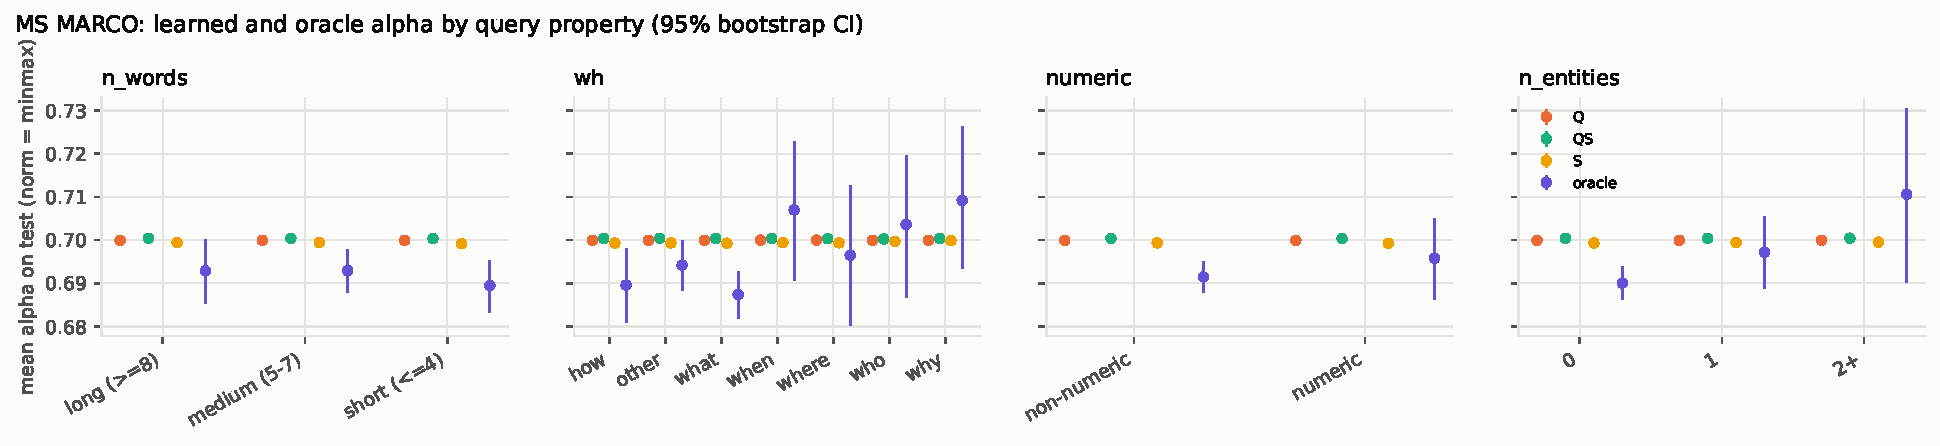
\includegraphics[width=\textwidth]{figures/diag_alpha_by_property.pdf}
  \caption{MS MARCO (A, test, min--max): mean learned $\alpha$ of the three gates and mean oracle
  $\alpha$ by query property, with 95\% bootstrap CIs. Learned $\alpha$ is constant; oracle $\alpha$ shows
  no trend in the predicted direction.}
  \label{fig:diag}
\end{figure*}
Before adding multi-hop data we checked whether ``$\alpha>0.5$ because MS MARCO queries are simple''
explains the MS MARCO result. CE-only beats GAT-only by only 1.6 nDCG@10 points on validation; the best
fixed $\alpha$ moves from 0.05 (none) to 0.70 (min--max, z-score) and 0.55 (rank), so its value is partly a
scale artefact; the learned $\alpha$ hardly varies (sd 0.0003--0.006); and its Spearman correlation with
query length and entity count is slightly \emph{positive} (+0.02 to +0.08), the opposite of the
prediction (Figure~\ref{fig:diag}). We recorded the explanation as not supported on MS MARCO and fixed
min--max as the primary normaliser.

\section{Reproducibility}
\label{app:repro}
All numbers are produced by the released pipeline (\texttt{python -m src.pipeline}); this report is
generated from its result files by \texttt{python -m src.report\_analysis} and
\texttt{python -m src.report\_paper}. Software: PyTorch 2.15, PyTorch Geometric 2.8.1,
sentence-transformers 6.2, Pyserini 1.6 (Lucene BM25 indexes \texttt{msmarco-v1-passage} and
\texttt{beir-v1.0.0-hotpotqa.flat}), ir\_datasets 0.6.3, ir\_measures 0.4.3, spaCy 3.8 with
\texttt{en\_core\_web\_sm}. Hardware: one NVIDIA RTX 6000 Ada (48\,GB). The complete multi-hop extension
(golden regression of MS MARCO, four datasets, graph controls, transfer, hypothesis tests) ran in
1~h~22~min; the MS MARCO study in under an hour. A golden regression confirmed that the variable-length
(masked) code reproduces all $2\times182$ MS MARCO runs exactly (maximum per-query difference $3\times10^{-8}$).
Deviations from the original protocol (e.g.\ the per-query $k$-NN graph instead of ReGAT-BERT's
structural graph, padding of short BM25 runs, a learnable bias in the BCE row) are logged in the
repository's \texttt{NOTES.md}.

\end{document}
